%!TEX root = ../TTK4550-MHT.tex
\section{Results}
\label{sec:results}

\subsection{Testing scheme}
The evaluation of the MHT algorithm is two-sided, firstly the algorithm must be able to track under challenging conditions, secondly it must be able to do this without having an ever growing computationally cost. The first performance metric is how well the algorithm is estimating the true position to the object it is tracking. This is measured as the Euclidean distance:
\begin{equation}
	\Delta P = \| \V{p}_{track}-\V{p}_{target} \|_2
\end{equation}
where the track is considered correct if $\Delta P \leq	\varepsilon_p$ for all t after initial convergence. If a track is deviating more that the threshold and is never within the threshold again, it is considered lost at the time-step it exceeded the threshold. If the track should converge after exceeding the threshold, it is considered restored at the time-step it is returning within the limit. The algorithm is tested on five scenarios:
\begin{itemize}
	\item Five fully cooperating ships
    \item Five partially cooperative ships
    \item Five ships avoiding obstacles with large space
    \item Five ships avoiding obstacles with little space
	\item Five parallel ships
\end{itemize}

\begin{figure}
    \centering
    \begin{subfigure}{0.49\textwidth}
        \centering
        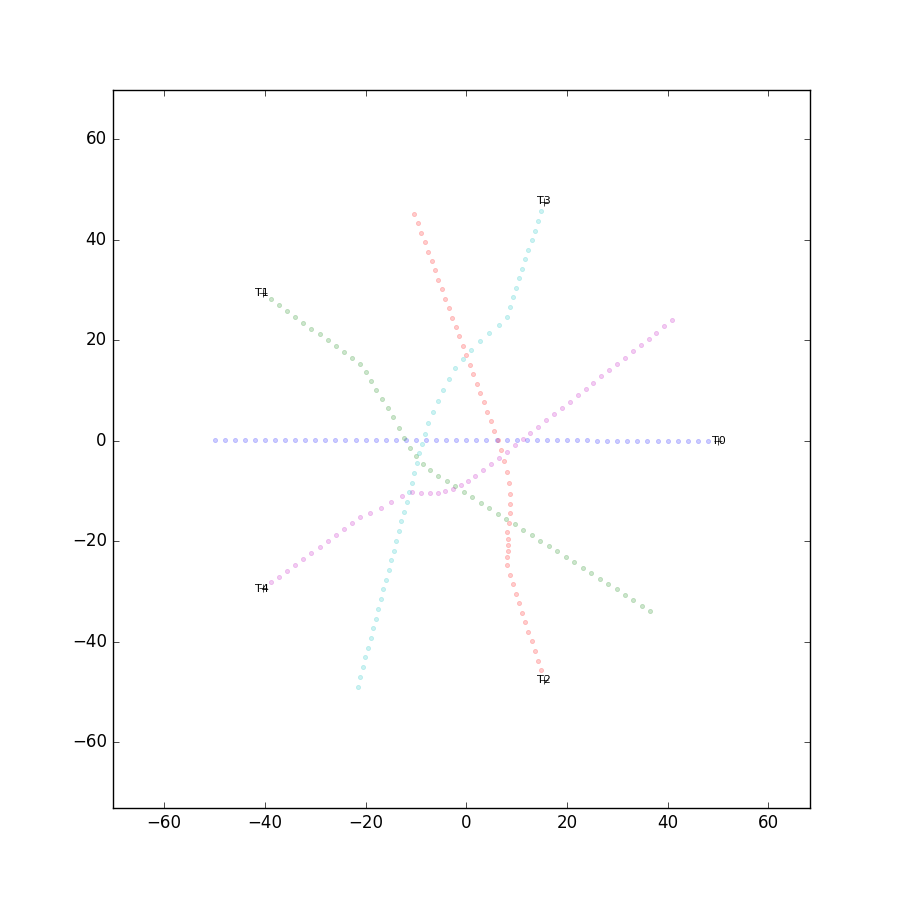
\includegraphics[height=0.3\textheight]{scenario1}
        \caption{First scenario}
    \end{subfigure}
    \begin{subfigure}{0.49\textwidth}
        \centering
        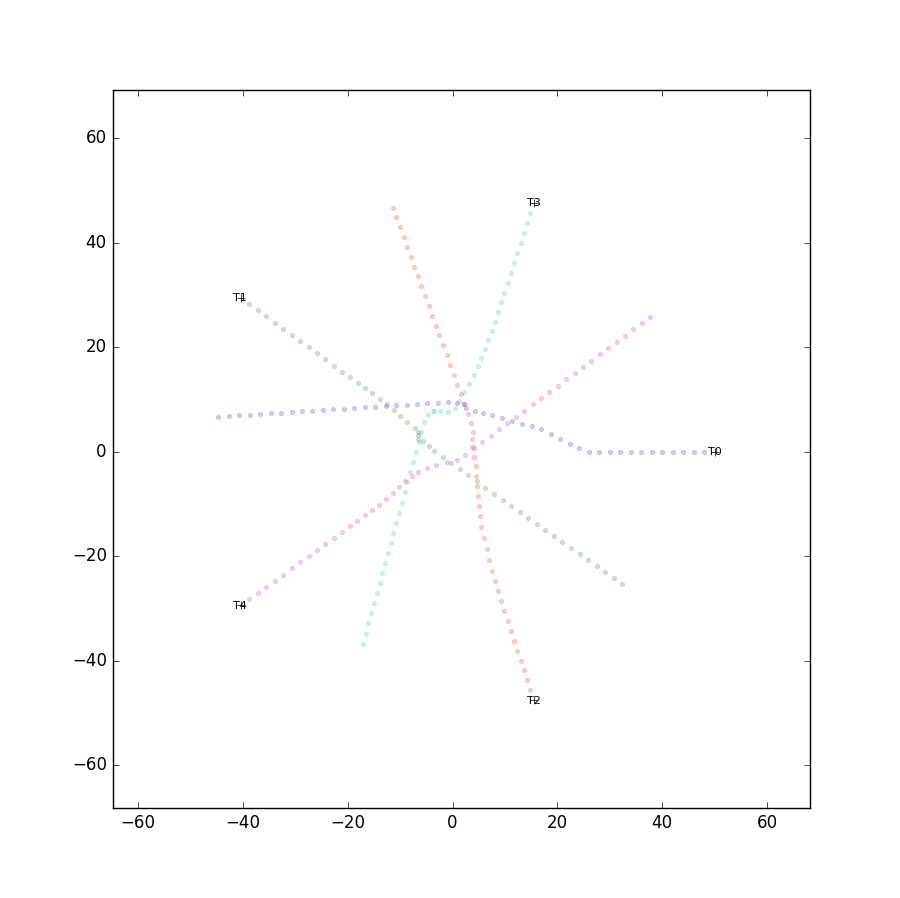
\includegraphics[height=0.3\textheight]{scenario2}
        \caption{Second scenario}
    \end{subfigure}
    \begin{subfigure}{0.49\textwidth}
        \centering
        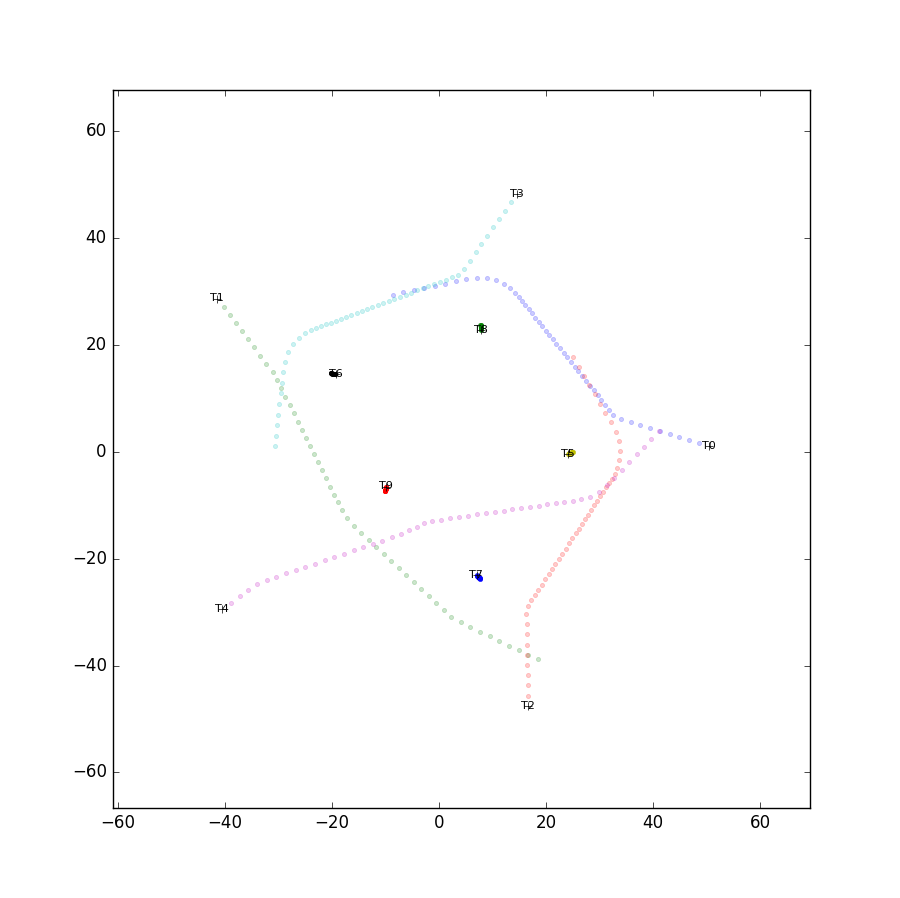
\includegraphics[height=0.3\textheight]{scenario3}
        \caption{Third scenario}
    \end{subfigure}
    \begin{subfigure}{0.49\textwidth}
        \centering
        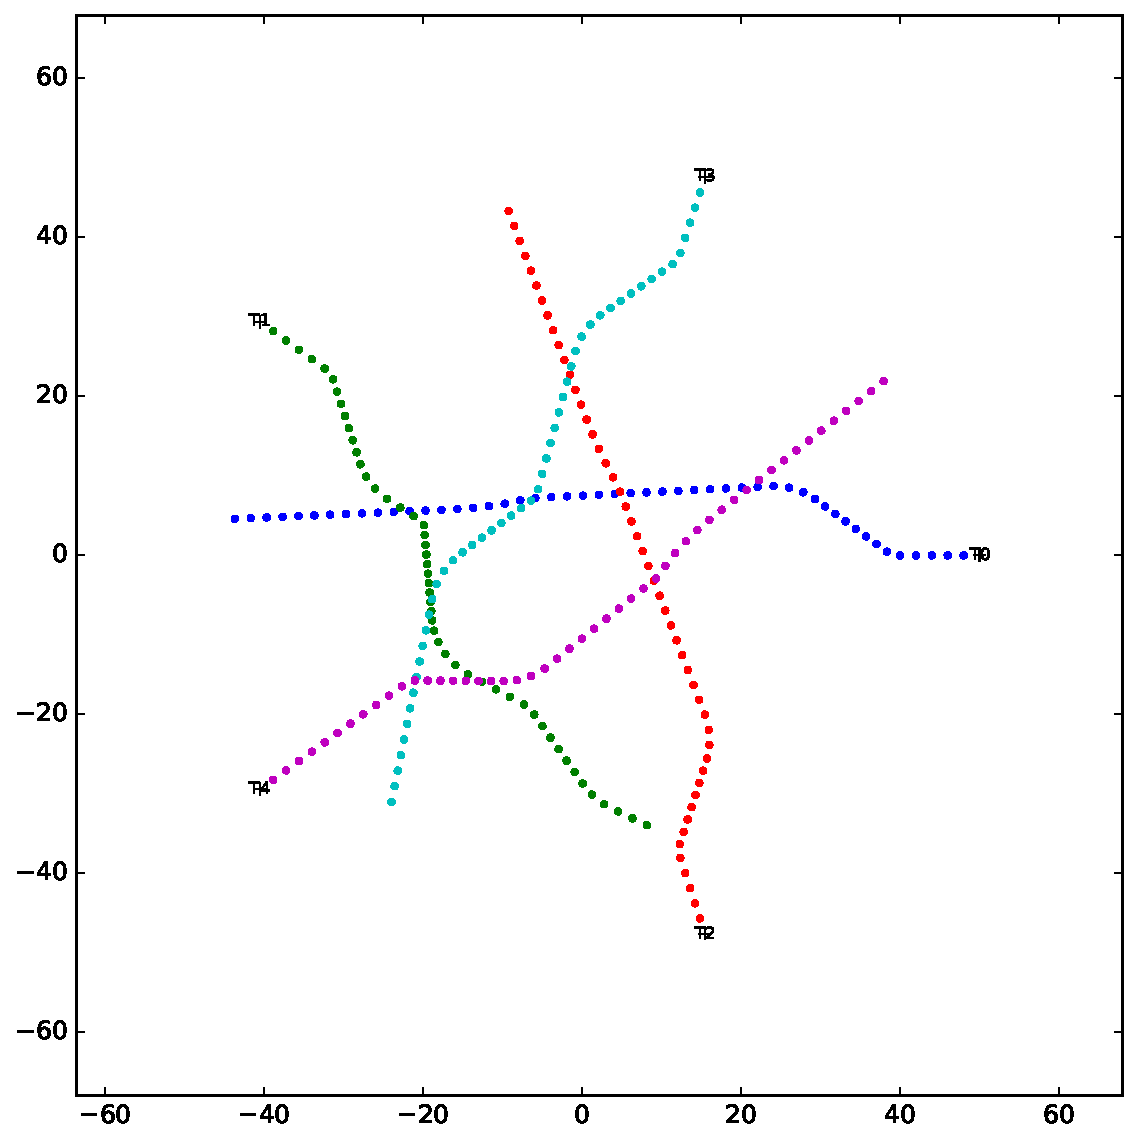
\includegraphics[height=0.3\textheight]{scenario4}
        \caption{Fourth scenario}
    \end{subfigure}
    \begin{subfigure}{0.49\textwidth}
        \centering
        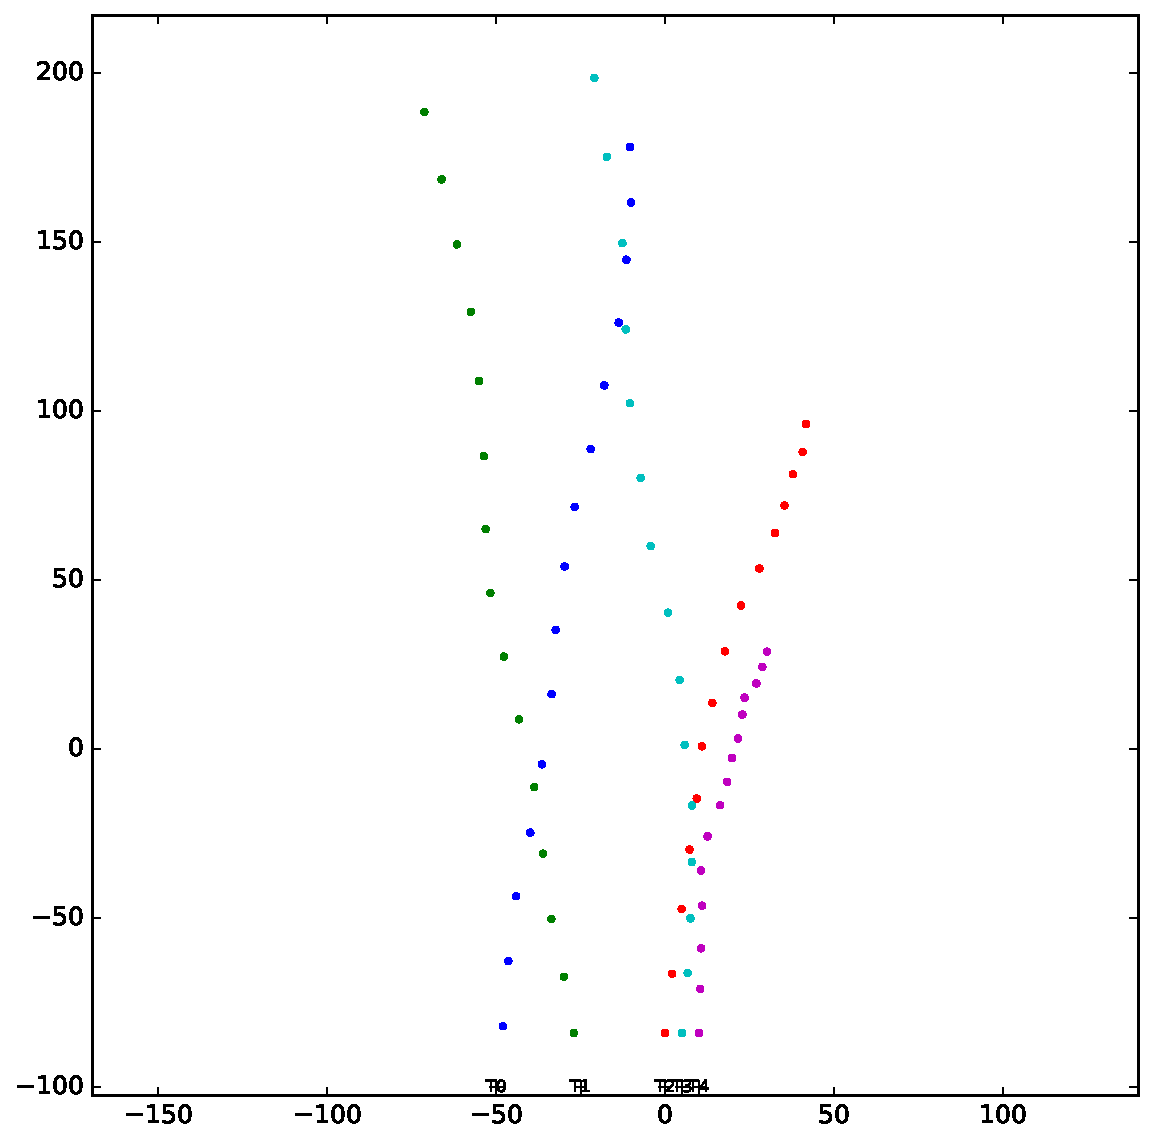
\includegraphics[height=0.29\textheight]{scenario5}
        \caption{Fifth scenario}
    \end{subfigure}
\end{figure}

\subsection{Simulation data}
Scenario one through four is generated as a recording of time and position from an Autonomous Surface Vessel (ASV)-simulator with collision avoidance (COLAV) which is a project under work by D. Kwame Minde Kufolaor at NTNU. The targets are configured such that they need to maneuver to avoid collision with each other, which allows for tracking of maneuvering targets in close proximity to each other. These scenarios where sampled at 1 Hz which is a little faster than a normal high speed vessel radar at 0.8 Hz (48 rpm). The fifth scenario is generated as a part of this project and is composed by linear parallel paths with white Gaussian system noise as maneuvering. This data set where sampled at 0.5 Hz which is a little higher that a normal maritime costal radar at 0.4 Hz (24 rpm).

\subsection{Simulations}
Scenario one through four was simulated with the following variations with all four solvers.
\begin{equation*}
\begin{split}
\V{P_D} &= \begin{bmatrix} 0.5 & 0.6 & 0.7 & 0.8 & 0.9 \end{bmatrix} \\
\V{N} &=\begin{bmatrix} 1 & 3 & 6 \end{bmatrix} \\
\V{\lambda_\phi} &=\begin{bmatrix} 0 & 1\cdot10^{-4} & 2\cdot10^{-4} & 4\cdot10^{-4} & 8\cdot10^{-4} \end{bmatrix}
\end{split}
\end{equation*}
Each variant was simulated 100 times with different seeded random clutter measurements and miss detections. For each simulation, the estimated tracks where compared with the true tacks and categorised in successful and lost tracks, the track loss threshold $\epsilon_p$ was $4$ meters. Figure \ref{fig:dynamic_agents_full_cooperation_cropped} - \ref{fig:dynamic_and_static_agents_narrow_space_cropped} show the averaged track loss percentage.

\subsubsection{Tracking performance}
\begin{figure}[H]
    \centering
    \textbf{Scenario 1}\par \medskip
    \begin{subfigure}{0.49\textwidth}
        \centering
        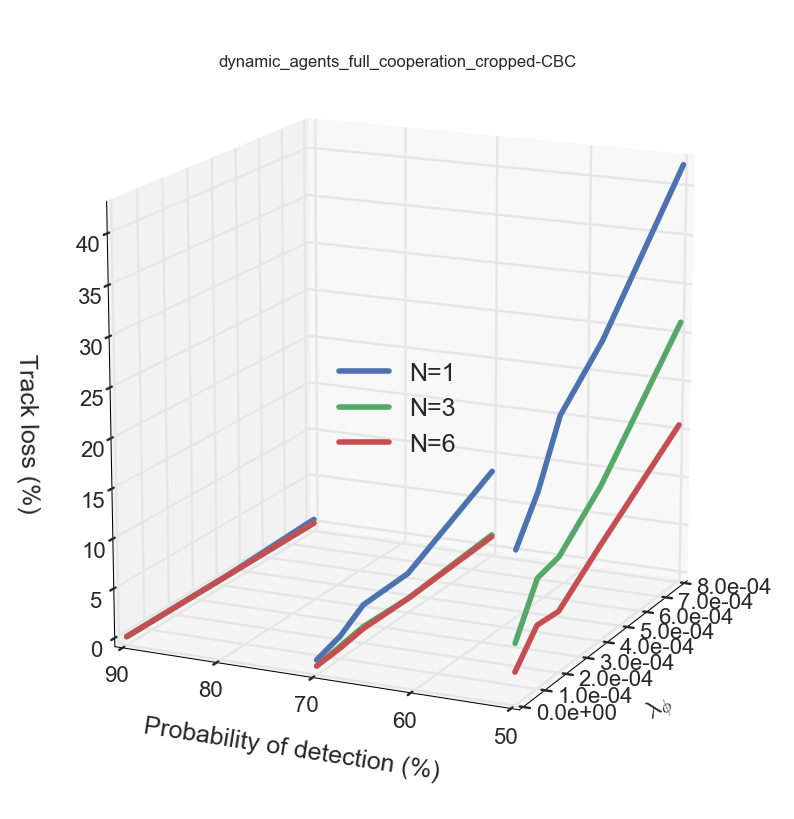
\includegraphics[clip, trim=0cm 0cm 0cm 2cm, width=\textwidth]{dynamic_agents_full_cooperation_cropped-CBC}
        \caption{CBC solver}
    \end{subfigure}
    \begin{subfigure}{0.49\textwidth}
        \centering
        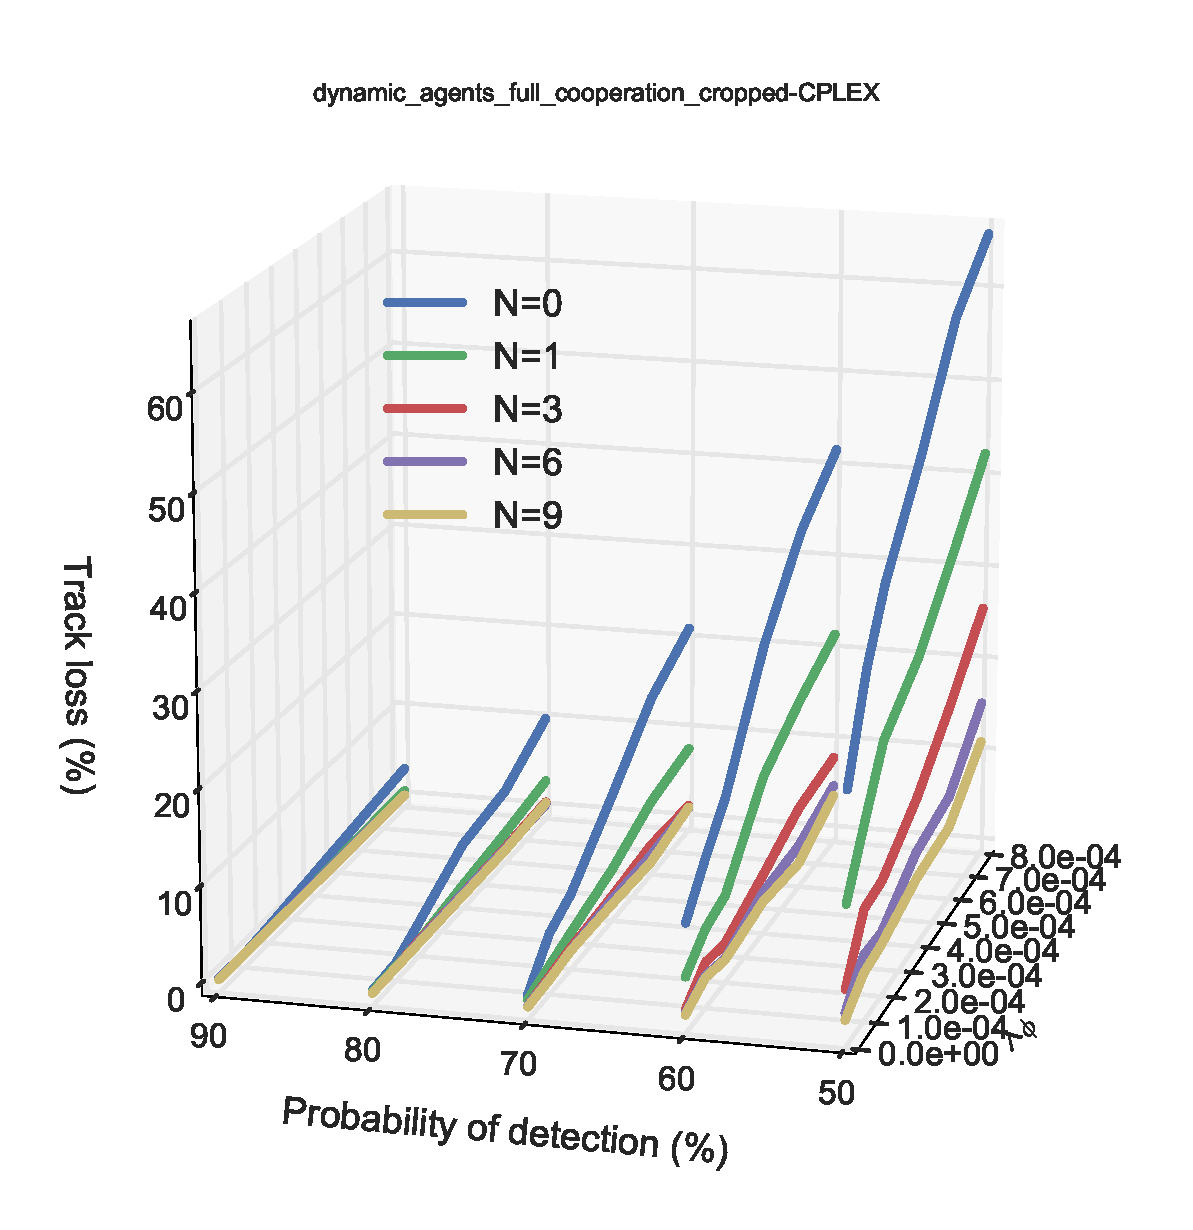
\includegraphics[clip,  trim=0cm 0cm 0cm 2cm,width=\textwidth]{dynamic_agents_full_cooperation_cropped-CPLEX}
        \caption{CPLEX solver}
    \end{subfigure}
    \begin{subfigure}{0.49\textwidth}
        \centering
        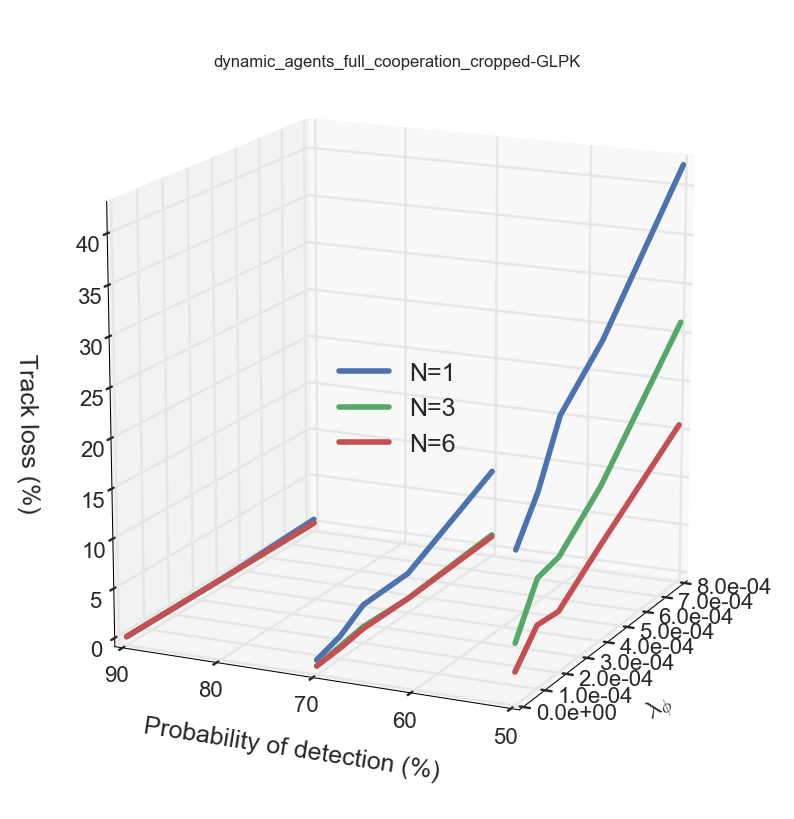
\includegraphics[clip,  trim=0cm 0cm 0cm 2cm,width=\textwidth]{dynamic_agents_full_cooperation_cropped-GLPK}
        \caption{GLPK solver}
    \end{subfigure}
    \begin{subfigure}{0.49\textwidth}
        \centering
        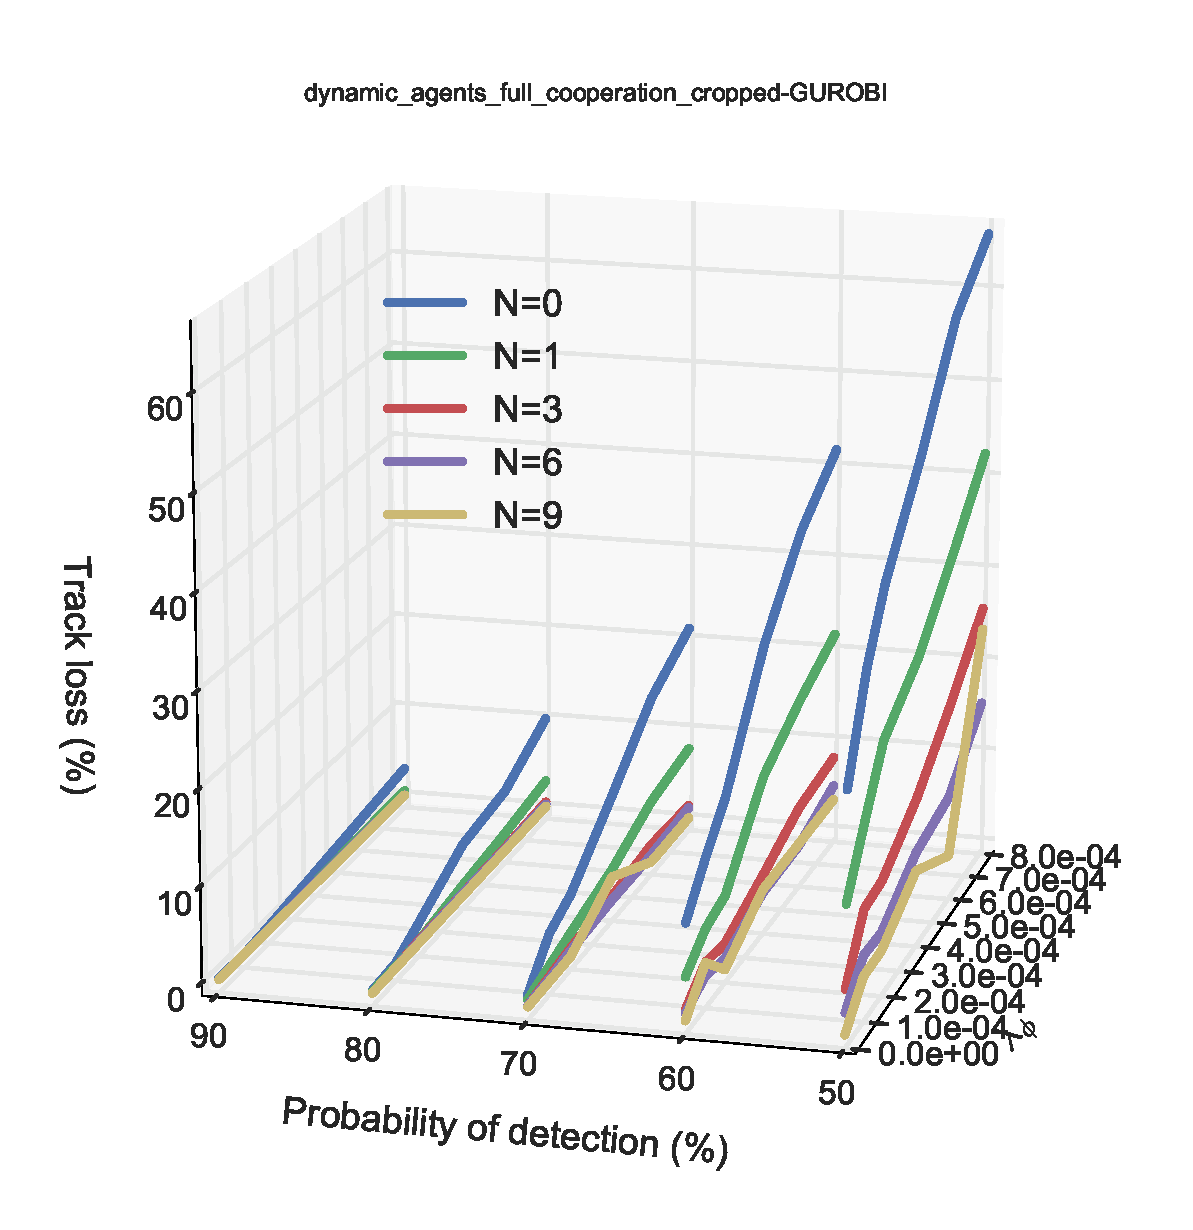
\includegraphics[clip,  trim=0cm 0cm 0cm 2cm,width=\textwidth]{dynamic_agents_full_cooperation_cropped-GUROBI}
        \caption{GUROBI solver}
    \end{subfigure}
	\caption{Simulation results for all solvers in scenario 1}
    \label{fig:dynamic_agents_full_cooperation_cropped}
\end{figure}

\begin{figure}[H]
    \centering
    \textbf{Scenario 2}\par \medskip
    \begin{subfigure}{0.49\textwidth}
        \centering
        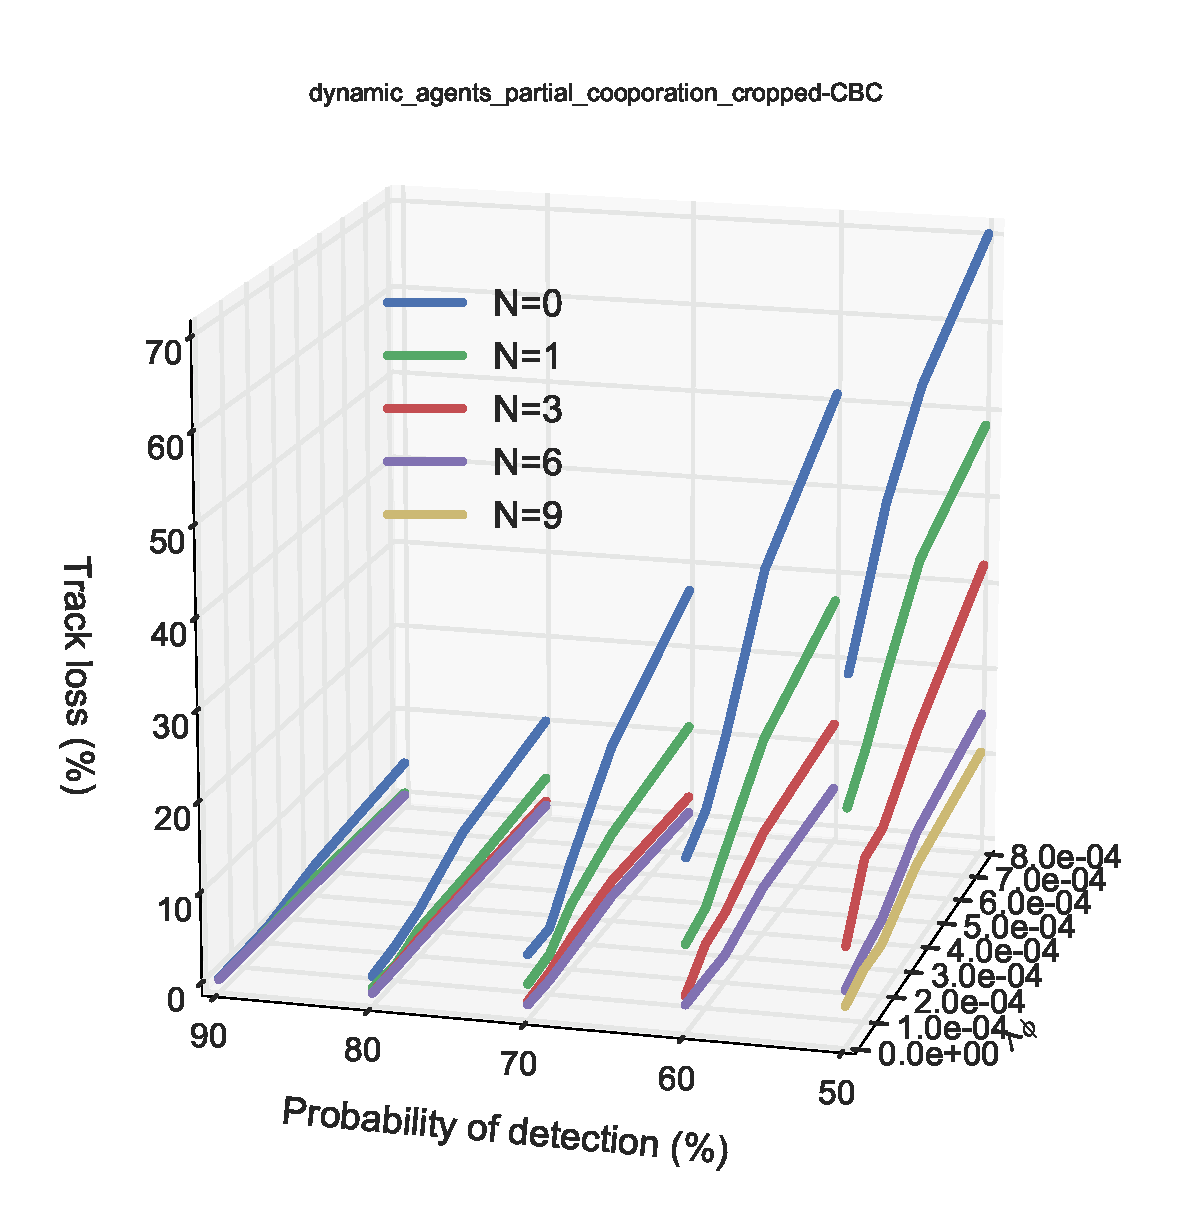
\includegraphics[clip,  trim=0cm 0cm 0cm 2cm, width=\textwidth]{dynamic_agents_partial_cooporation_cropped-CBC}
        \caption{CBC solver}
    \end{subfigure}
    \begin{subfigure}{0.49\textwidth}
        \centering
        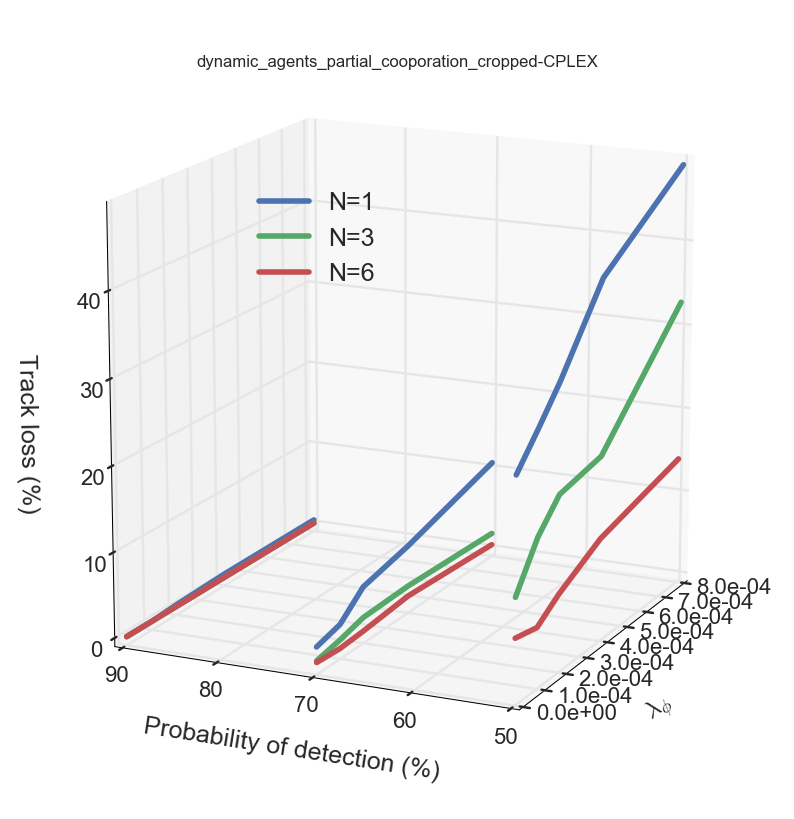
\includegraphics[clip,  trim=0cm 0cm 0cm 2cm,width=\textwidth]{dynamic_agents_partial_cooporation_cropped-CPLEX}
        \caption{CPLEX solver}
    \end{subfigure}
    \begin{subfigure}{0.49\textwidth}
        \centering
        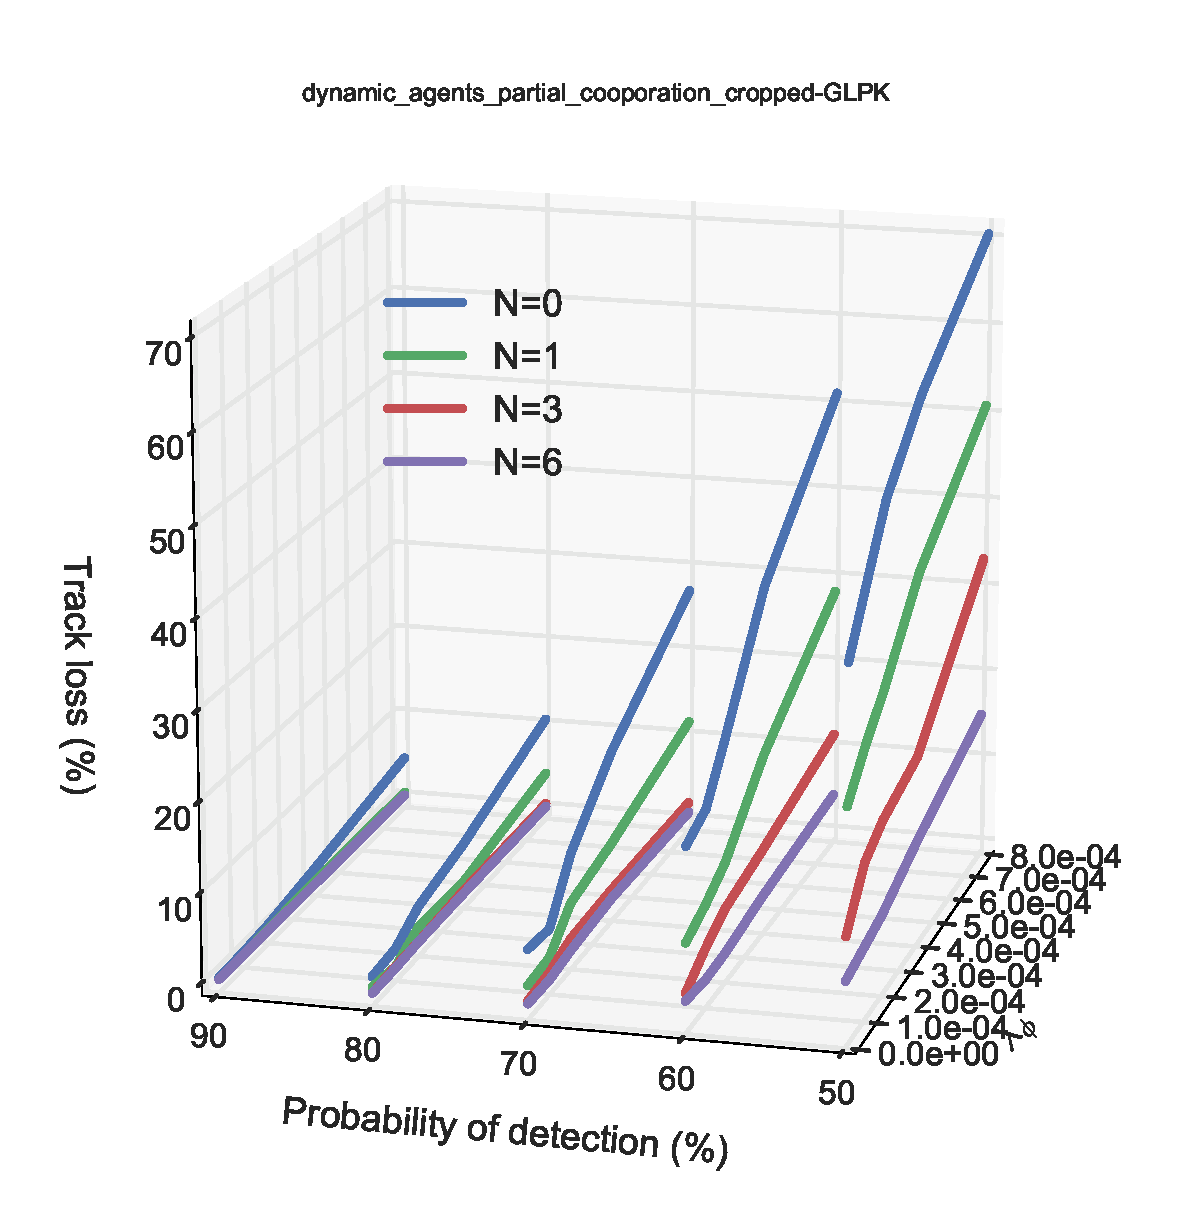
\includegraphics[clip,  trim=0cm 0cm 0cm 2cm,width=\textwidth]{dynamic_agents_partial_cooporation_cropped-GLPK}
        \caption{GLPK solver}
    \end{subfigure}
    \begin{subfigure}{0.49\textwidth}
        \centering
        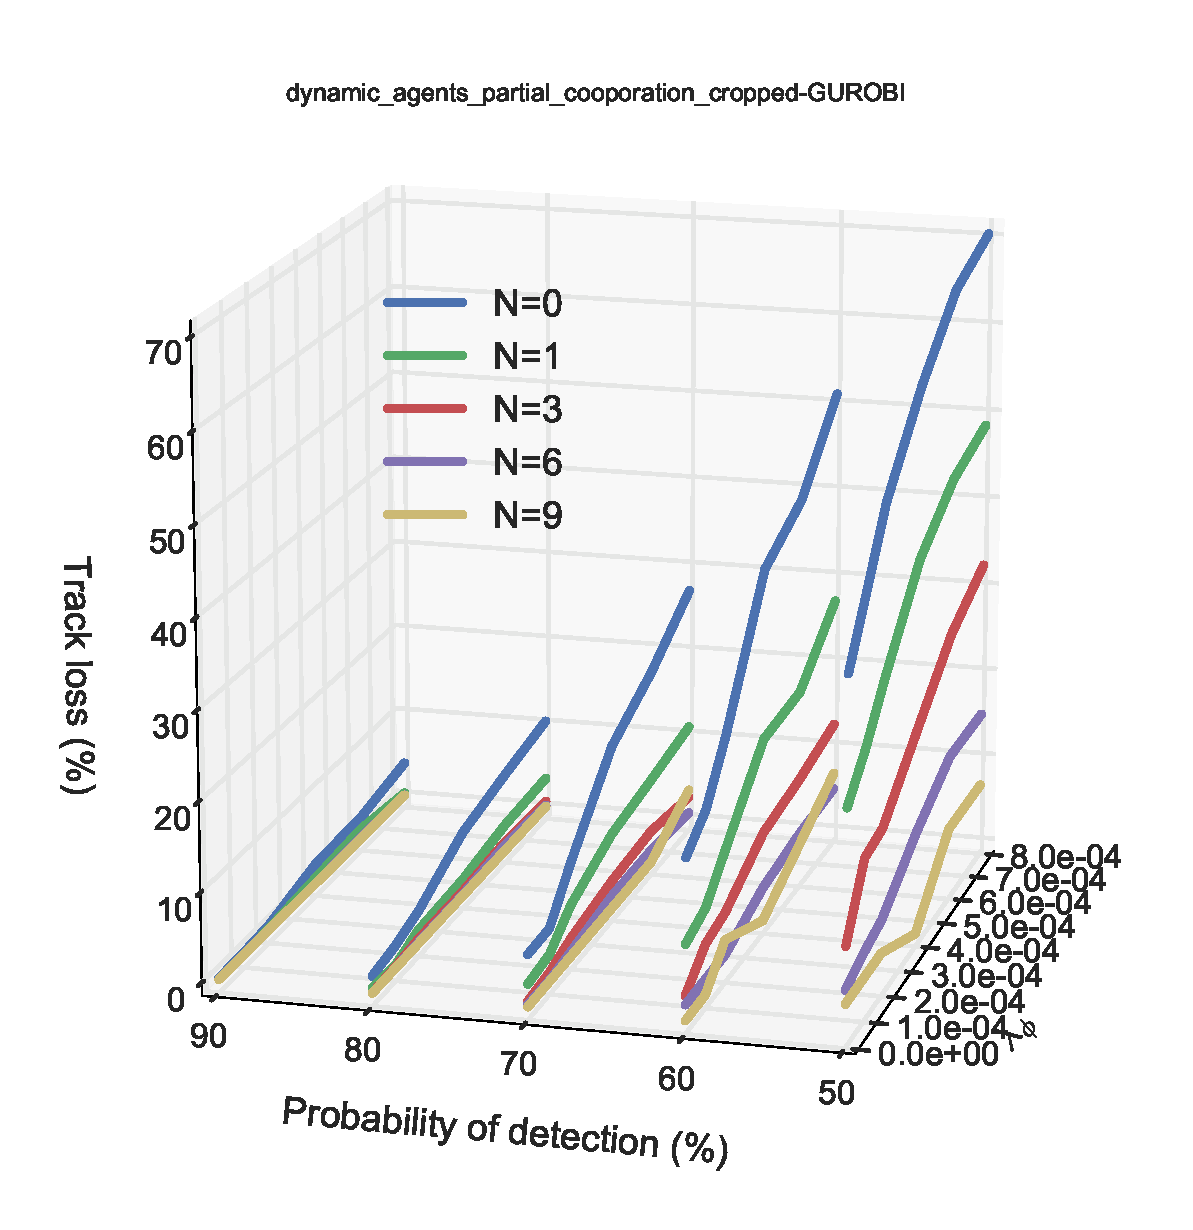
\includegraphics[clip, trim=0cm 0cm  0cm 2cm,width=\textwidth]{dynamic_agents_partial_cooporation_cropped-GUROBI}
        \caption{GUROBI solver}
    \end{subfigure}
    \caption{Simulation results for all solvers in scenario 2}
	\label{fig:dynamic_agents_partial_cooperation_cropped}
\end{figure}

\begin{figure}[H]
    \centering
    \textbf{Scenario3}\par \medskip
    \begin{subfigure}{0.49\textwidth}
        \centering
        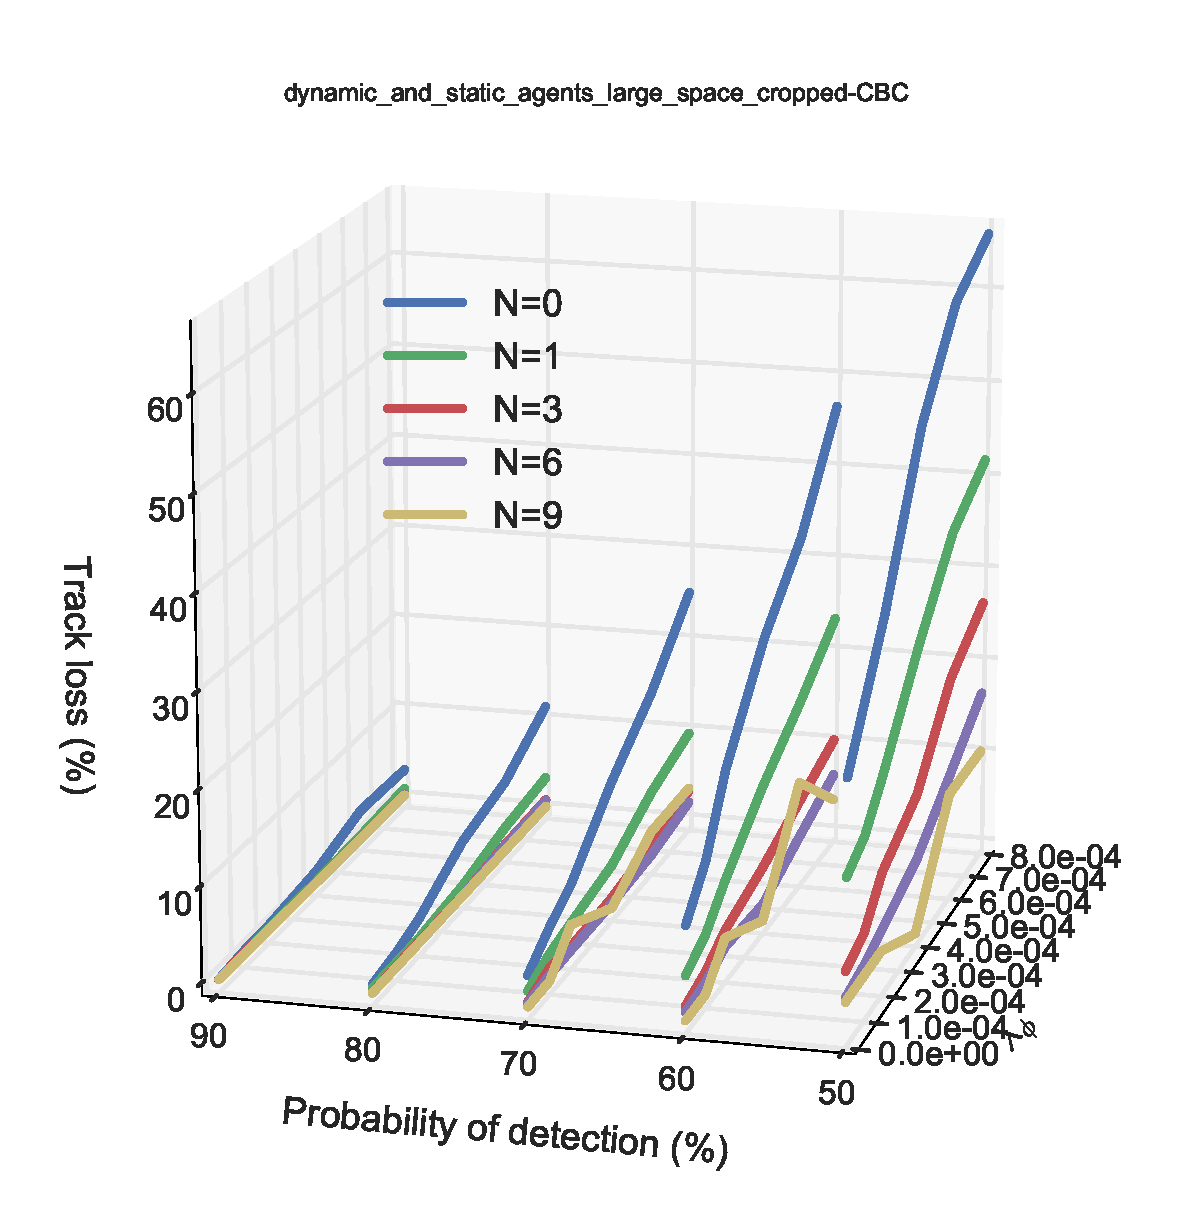
\includegraphics[clip, trim=0cm 0cm 0cm 2cm, width=\textwidth]{dynamic_and_static_agents_large_space_cropped-CBC}
        \caption{CBC solver}
    \end{subfigure}
    \begin{subfigure}{0.49\textwidth}
        \centering
        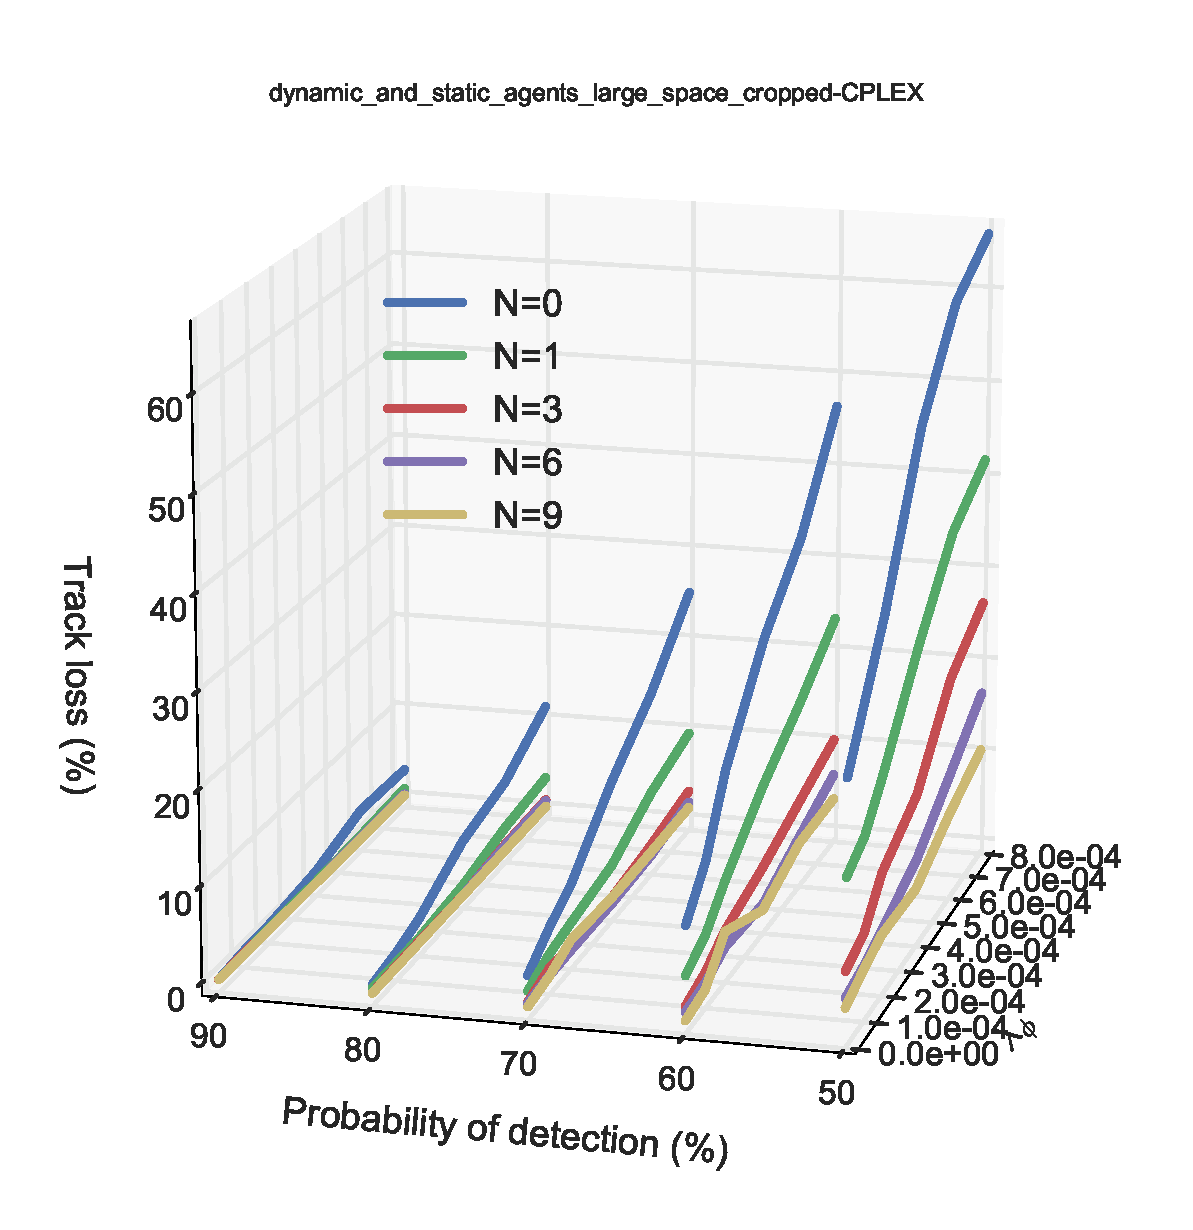
\includegraphics[clip, trim=0cm 0cm 0cm 2cm,width=\textwidth]{dynamic_and_static_agents_large_space_cropped-CPLEX}
        \caption{CPLEX solver}
    \end{subfigure}
    \begin{subfigure}{0.49\textwidth}
        \centering
        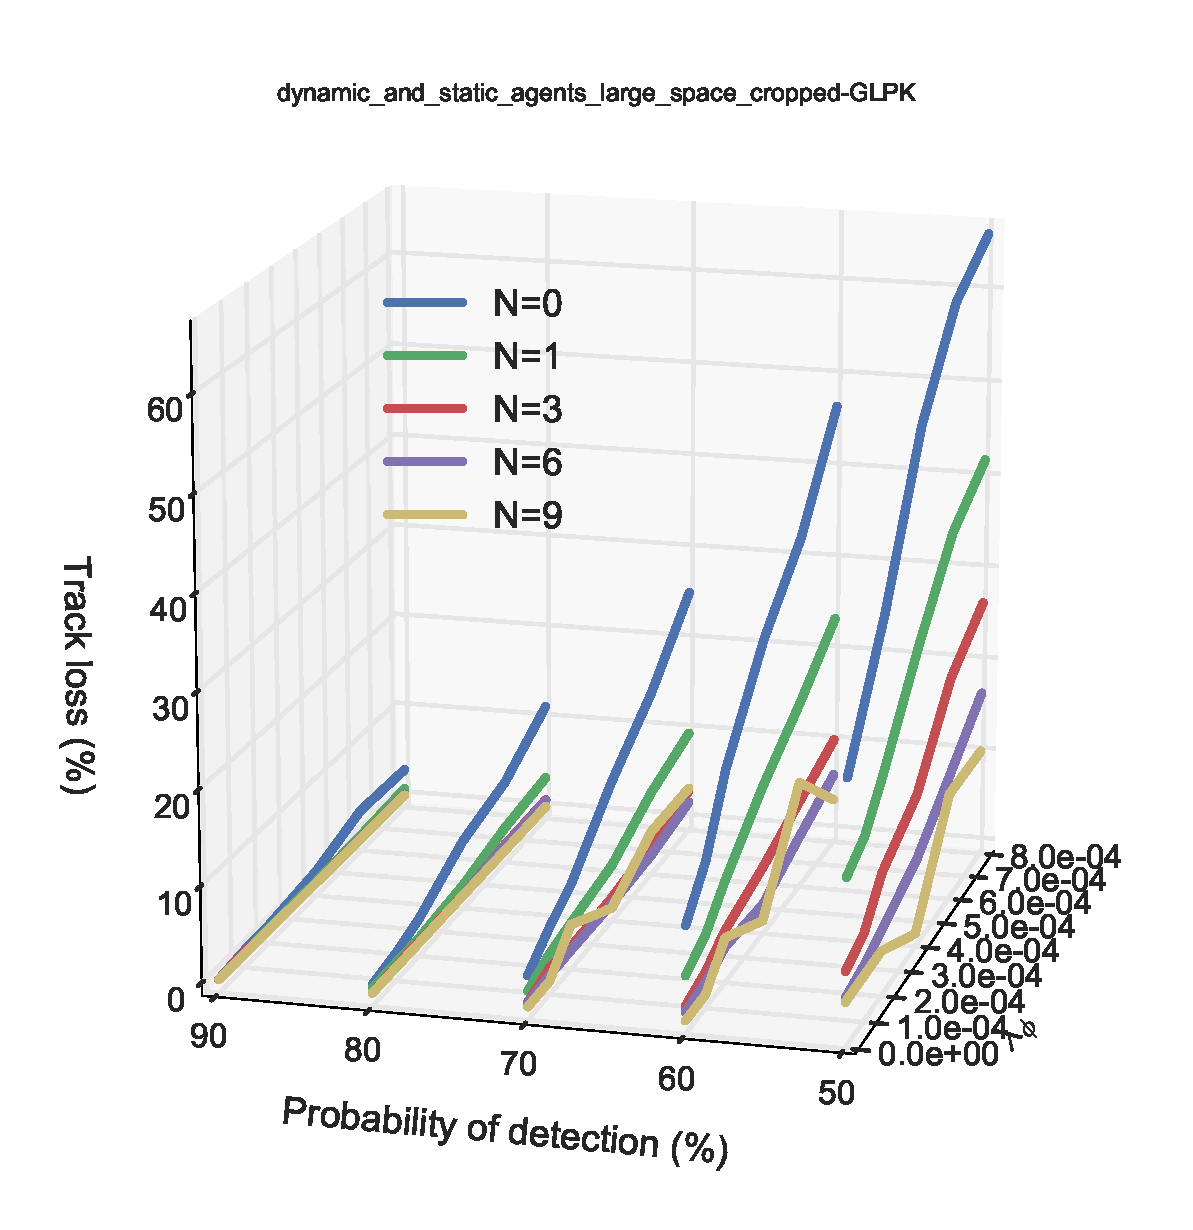
\includegraphics[clip, trim=0cm 0cm 0cm 2cm,width=\textwidth]{dynamic_and_static_agents_large_space_cropped-GLPK}
        \caption{GLPK solver}
    \end{subfigure}
    \begin{subfigure}{0.49\textwidth}
        \centering
        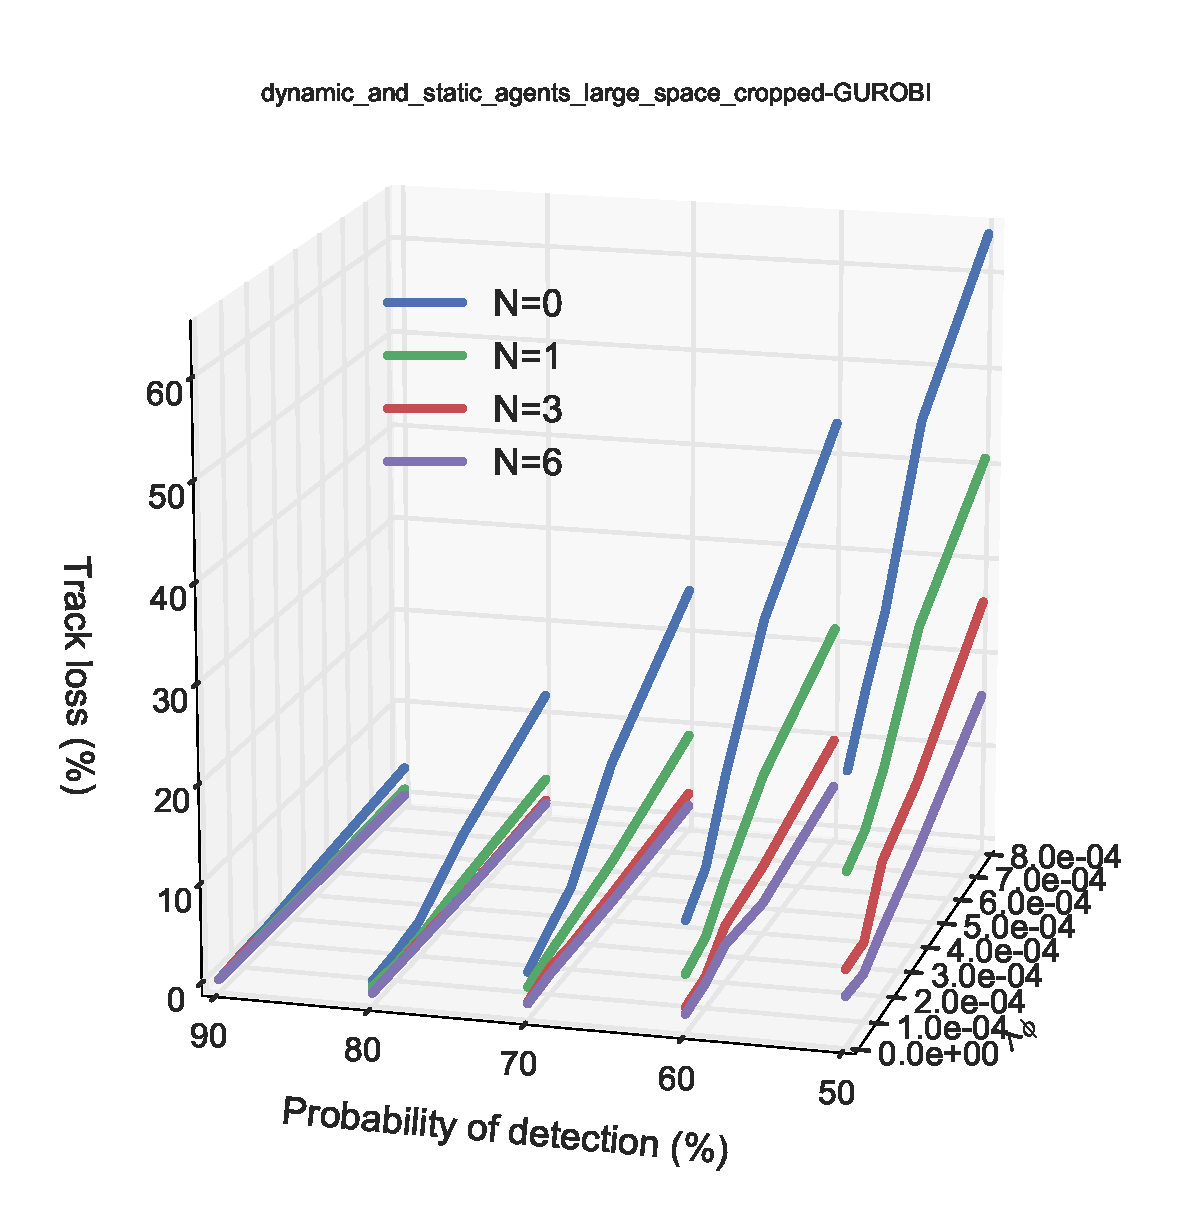
\includegraphics[clip, trim=0cm 0cm 0cm 2cm,width=\textwidth]{dynamic_and_static_agents_large_space_cropped-GUROBI}
        \caption{GUROBI solver}
    \end{subfigure}
    \caption{Simulation results for all solvers in scenario 3}
	\label{fig:dynamic_and_static_agents_large_space_cropped}
\end{figure}

\begin{figure}[H]
    \centering
    \textbf{Scenario 4}\par \medskip
    \begin{subfigure}{0.49\textwidth}
        \centering
        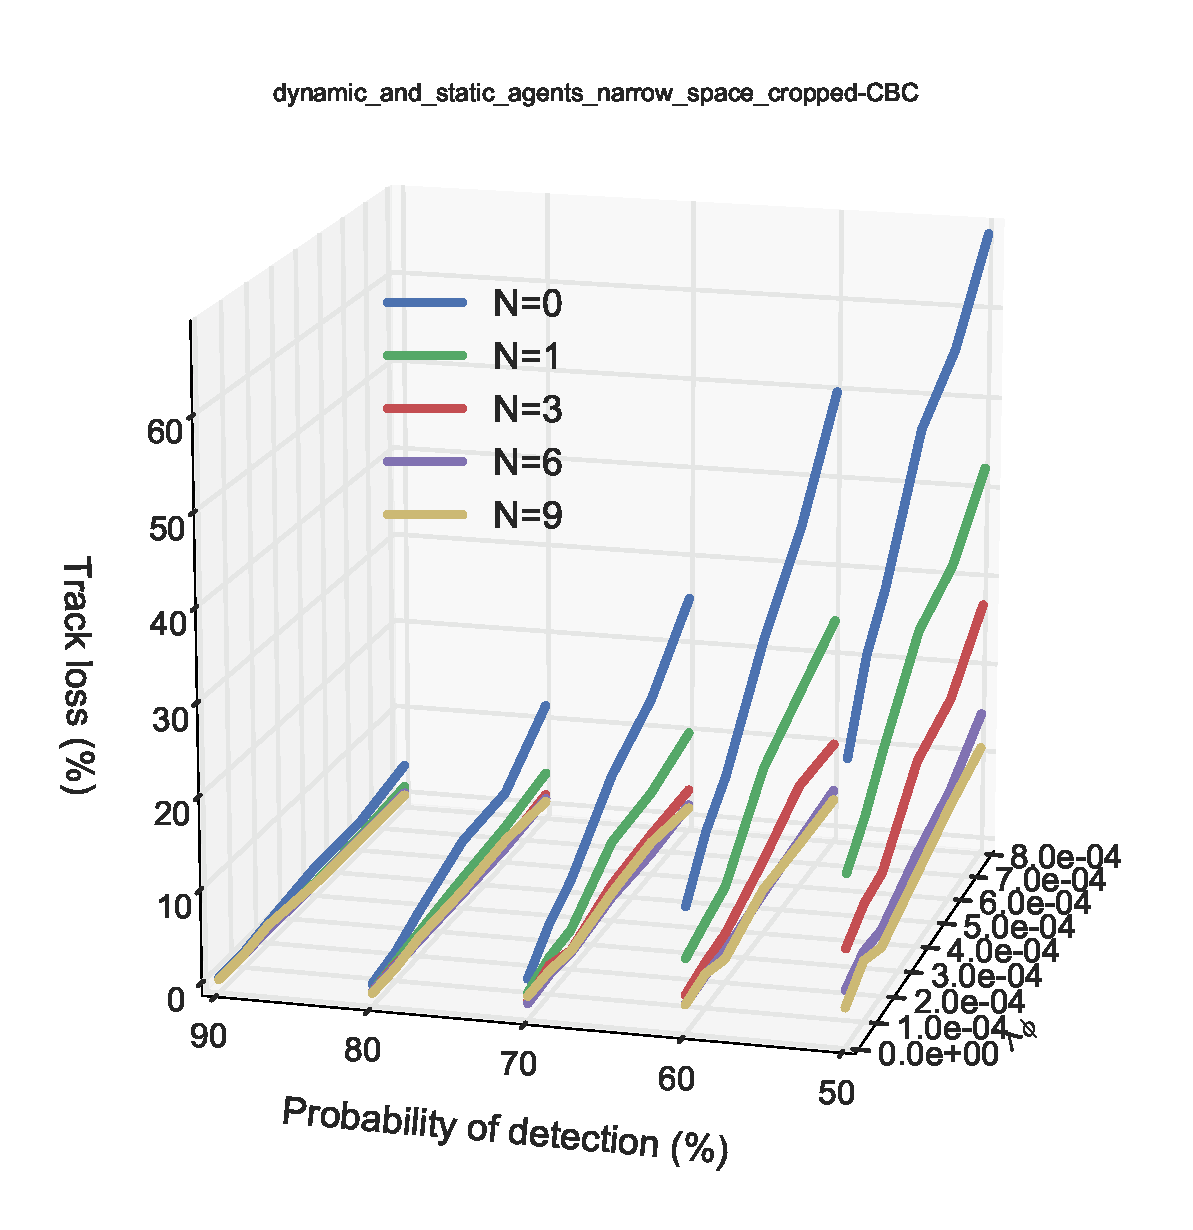
\includegraphics[clip,  trim=0cm 0cm 0cm 2cm, width=\textwidth]{dynamic_and_static_agents_narrow_space_cropped-CBC}
        \caption{CBC solver}
    \end{subfigure}
    \begin{subfigure}{0.49\textwidth}
        \centering
        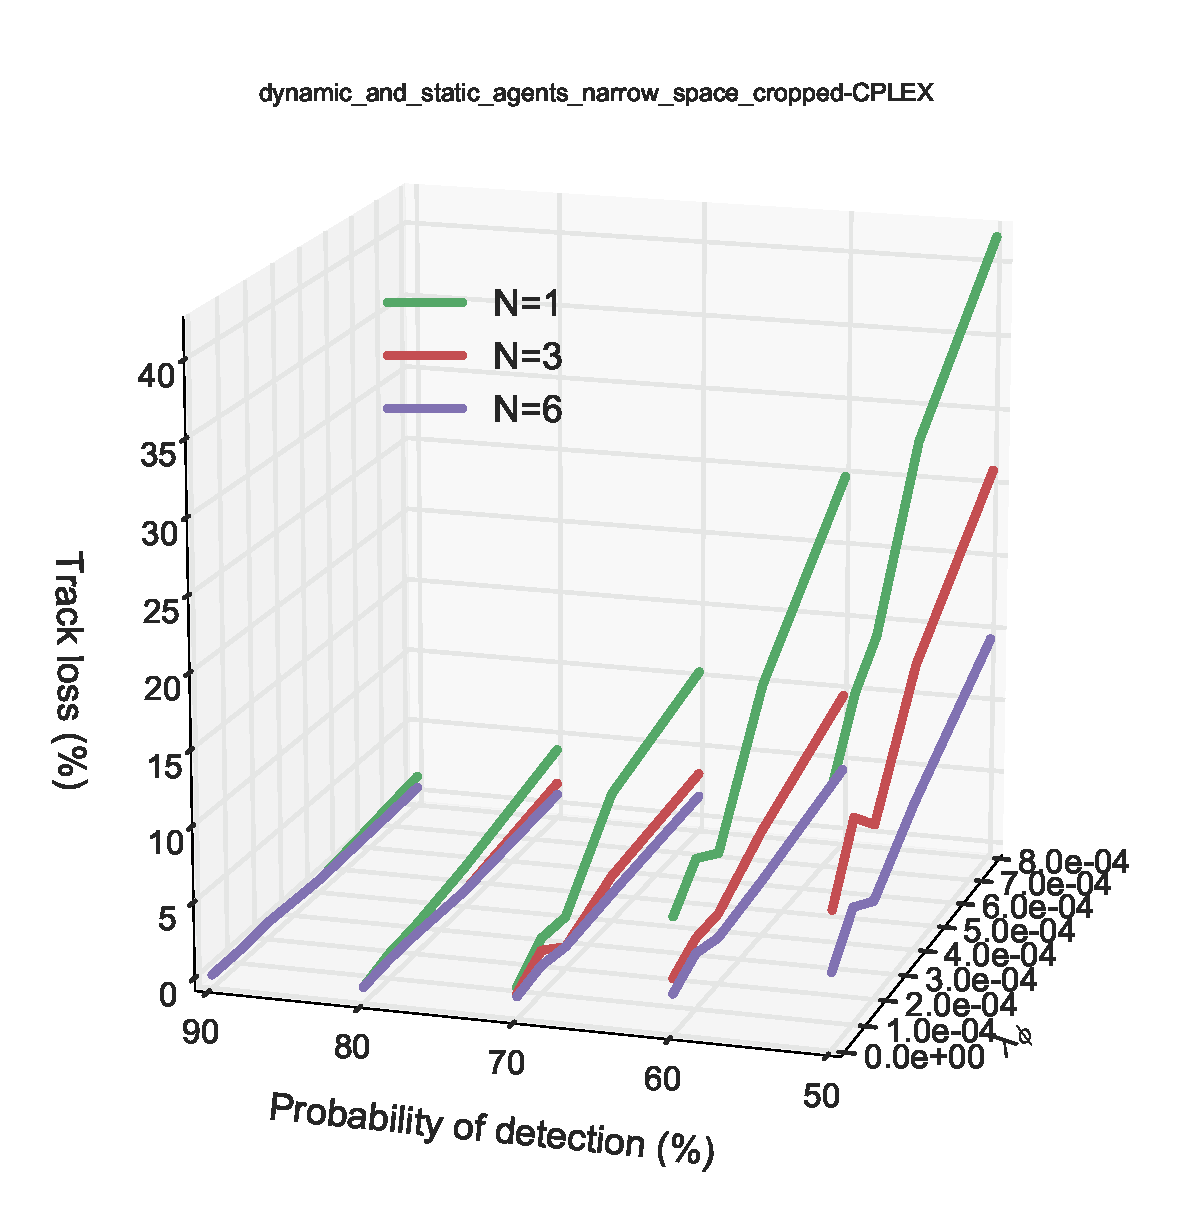
\includegraphics[clip, trim=0cm 0cm 0cm 2cm,width=\textwidth]{dynamic_and_static_agents_narrow_space_cropped-CPLEX}
        \caption{CPLEX solver}
    \end{subfigure}
    \begin{subfigure}{0.49\textwidth}
        \centering
        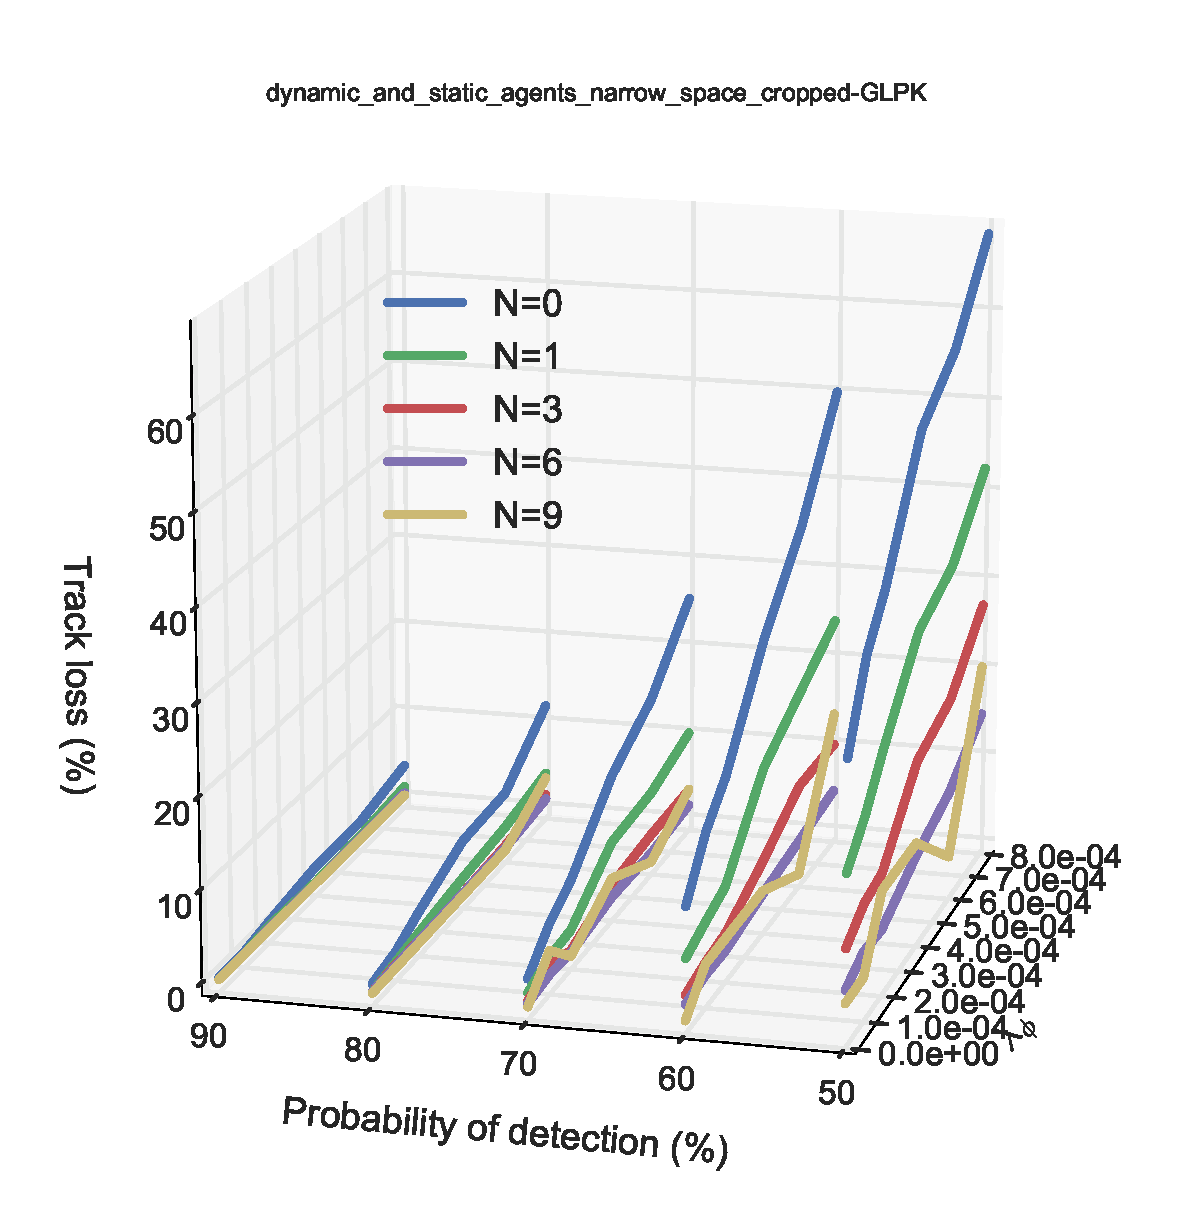
\includegraphics[clip, trim=0cm 0cm 0cm 2cm,width=\textwidth]{dynamic_and_static_agents_narrow_space_cropped-GLPK}
        \caption{GLPK solver}
    \end{subfigure}
    \begin{subfigure}{0.49\textwidth}
        \centering
        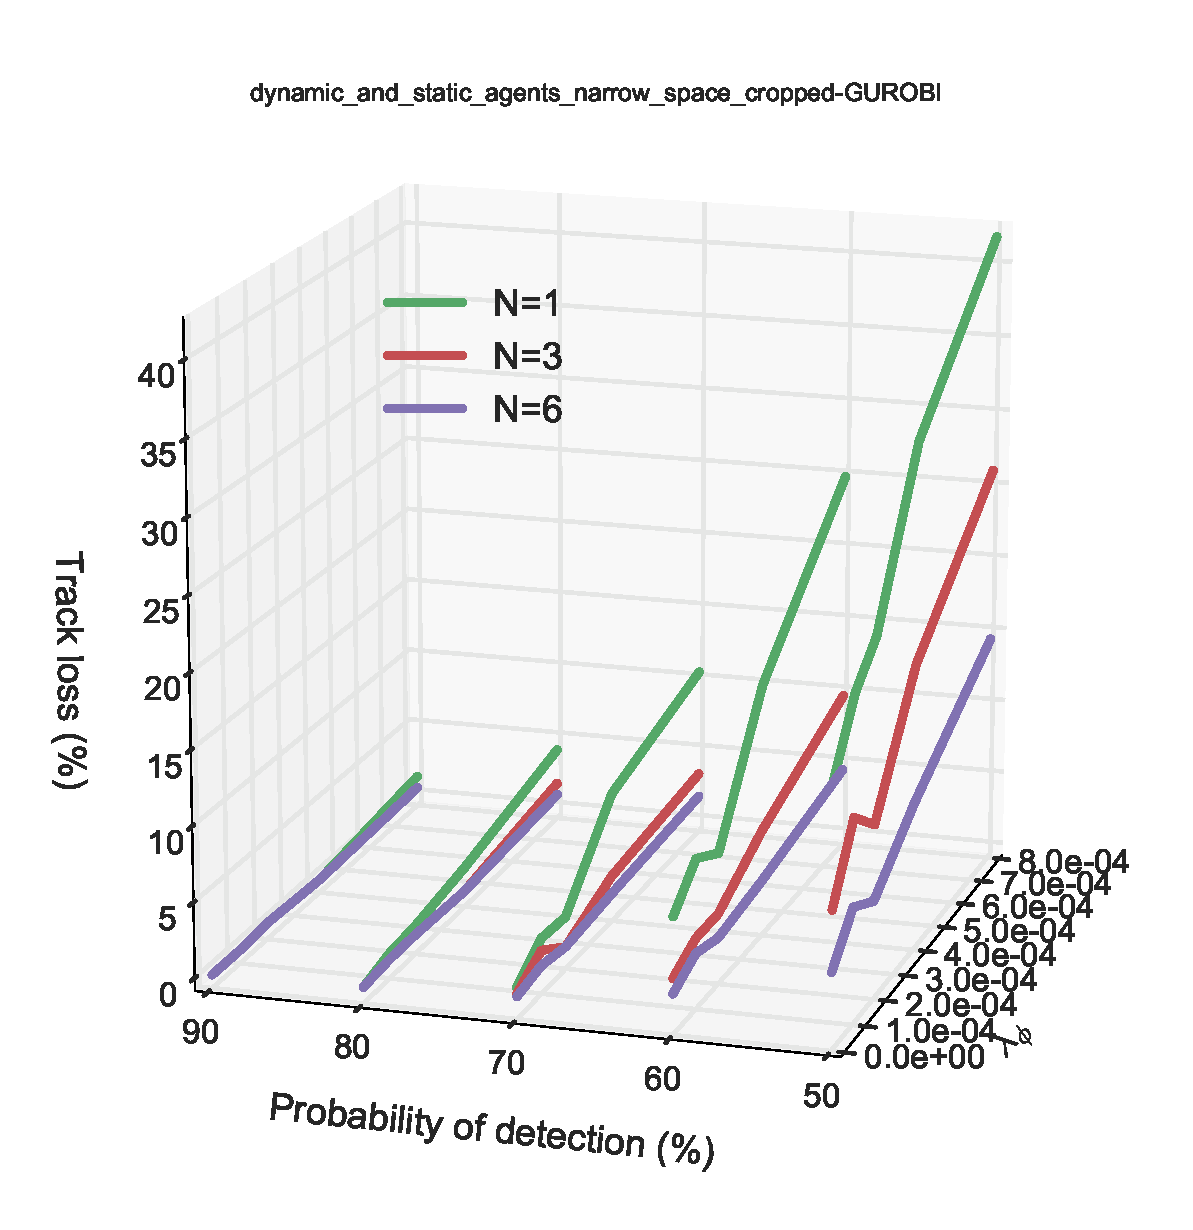
\includegraphics[clip, trim=0cm 0cm 0cm 2cm,width=\textwidth]{dynamic_and_static_agents_narrow_space_cropped-GUROBI}
        \caption{GUROBI solver}
    \end{subfigure}
    \caption{Simulation results for all solvers in scenario 4}
	\label{fig:dynamic_and_static_agents_narrow_space_cropped}
\end{figure}

\begin{figure}[H]
    \centering
    \textbf{Scenario 5}\par \medskip
    \begin{subfigure}{0.49\textwidth}
        \centering
        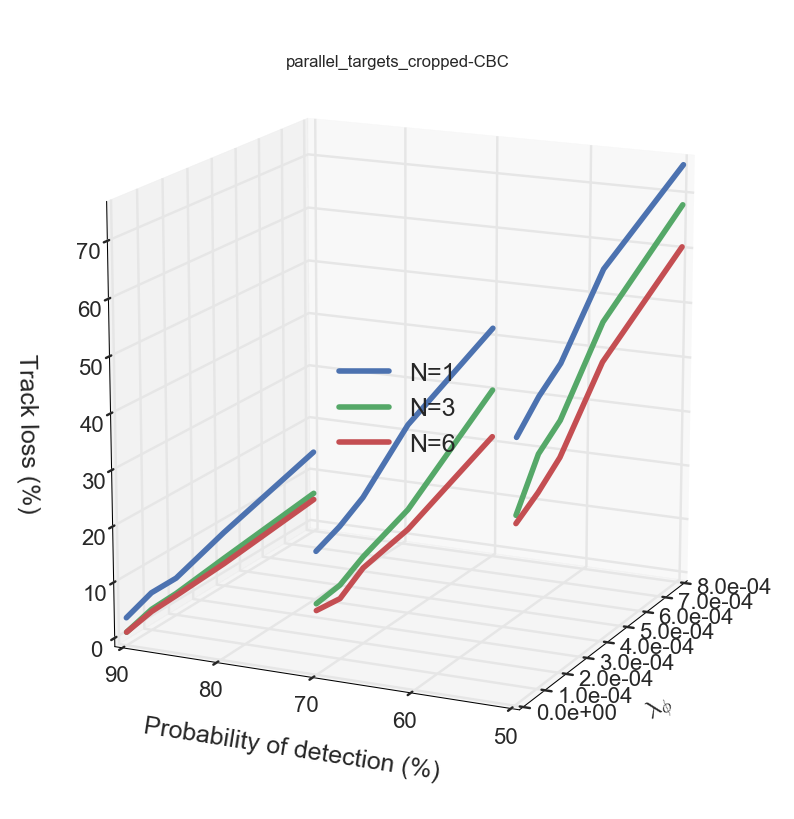
\includegraphics[clip,  trim=0cm 0cm 0cm 2cm, width=\textwidth]{parallel_targets_cropped-CBC}
        \caption{CBC solver}
    \end{subfigure}
    \begin{subfigure}{0.49\textwidth}
        \centering
        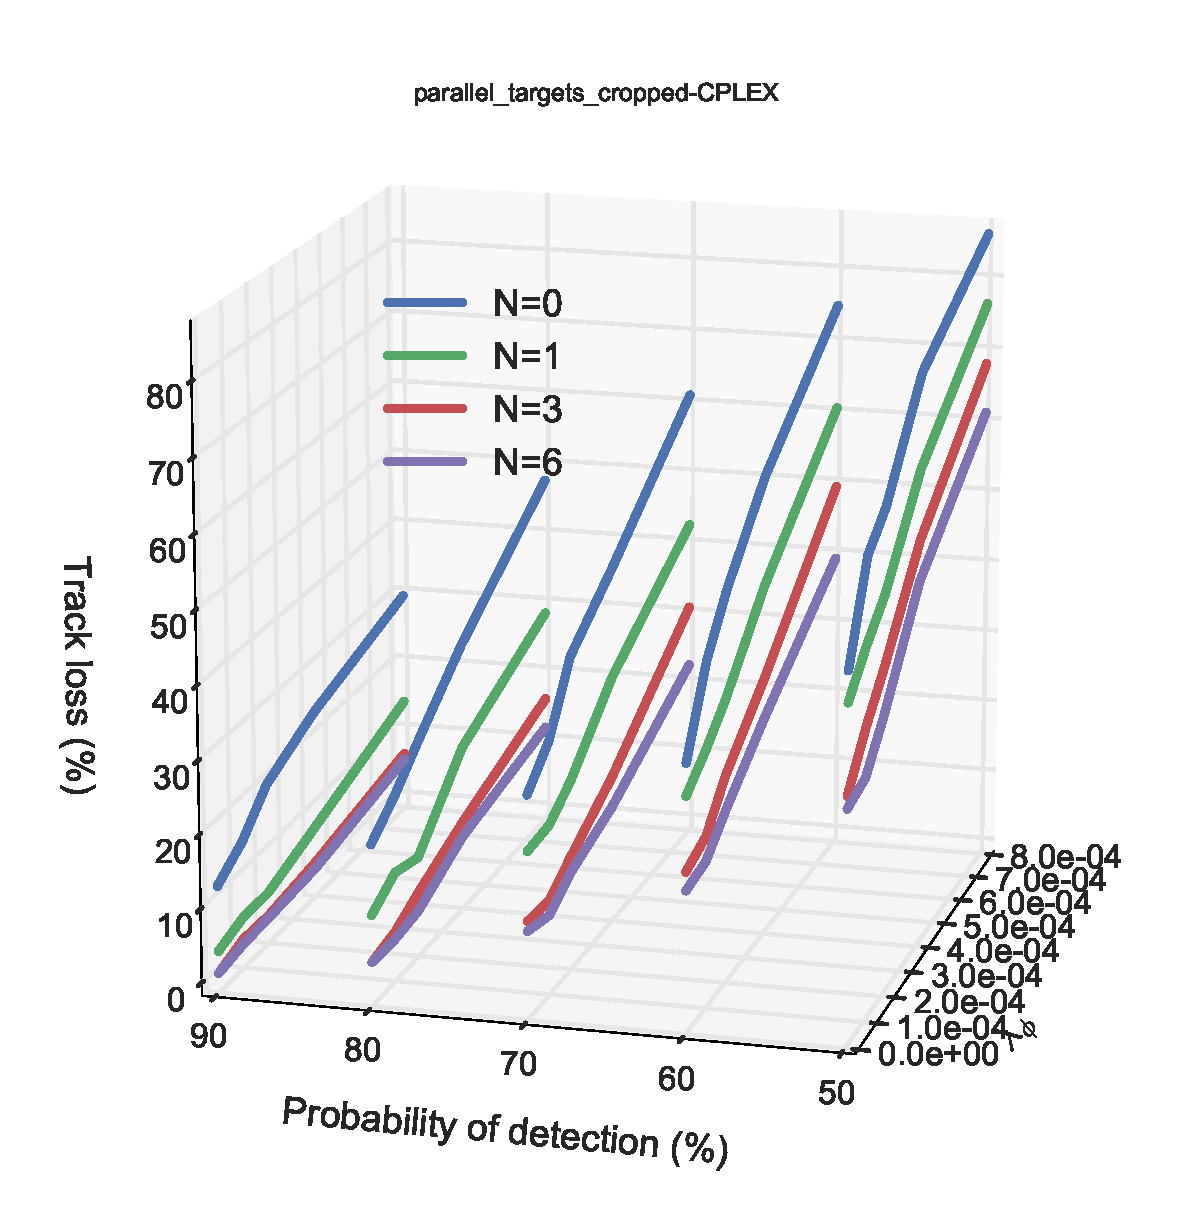
\includegraphics[clip, trim=0cm 0cm 0cm 2cm,width=\textwidth]{parallel_targets_cropped-CPLEX}
        \caption{CPLEX solver}
    \end{subfigure}
    \begin{subfigure}{0.49\textwidth}
        \centering
        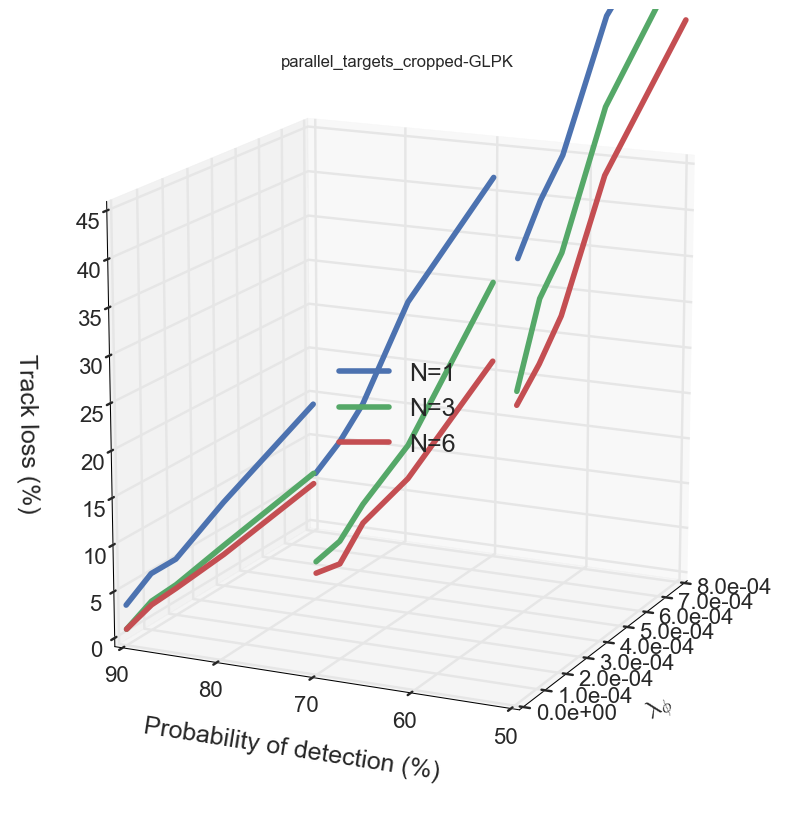
\includegraphics[clip, trim=0cm 0cm 0cm 2cm,width=\textwidth]{parallel_targets_cropped-GLPK}
        \caption{GLPK solver}
    \end{subfigure}
    \begin{subfigure}{0.49\textwidth}
        \centering
        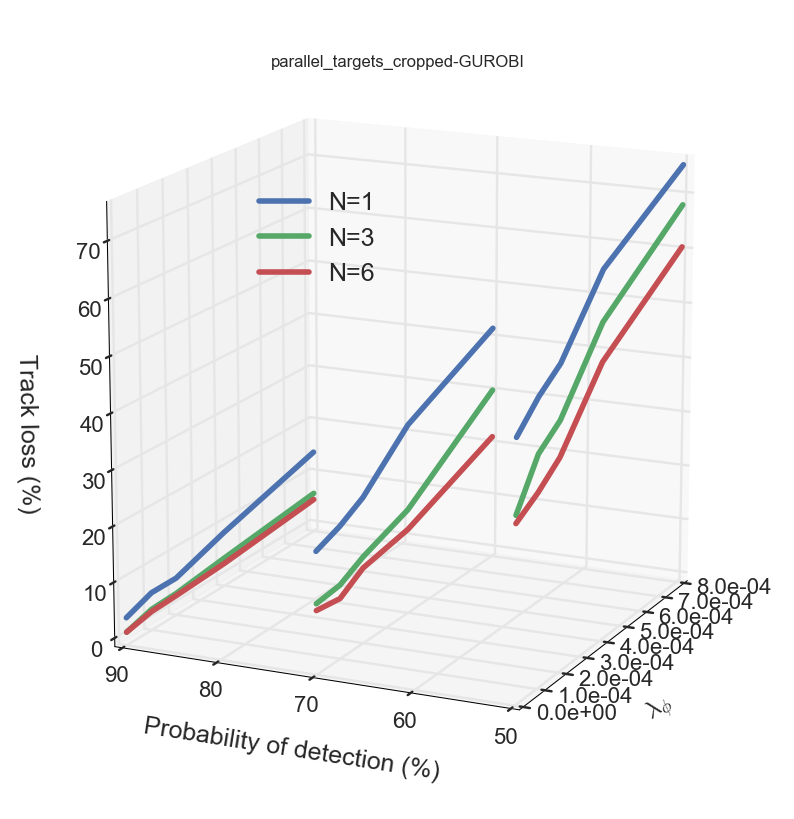
\includegraphics[clip, trim=0cm 0cm 0cm 2cm,width=\textwidth]{parallel_targets_cropped-GUROBI}
        \caption{GUROBI solver}
    \end{subfigure}
    \caption{Simulation results for all solvers in scenario 5}
    \label{fig:parallel_targets_cropped}
\end{figure} 
From the simulations it can be observed that the different solvers perform practically identically when it comes to track performance. The number of lost tracks is proportional with the clutter level at a rate which is inverse proportional with the probability of detection $P_D$. An interesting observation is the return on investment regarding the number of scans to evaluate (N-scan). For instance, with $P_D=0.7$ the difference between $N=3$ and $N=6$ is marginal, at least when the clutter level is within reasonable levels. With $P_D=0.5$ we see that the pay-off is much higher for the extra computational cost with 15\% improvement between $N=3$ and $N=6$.
\subsection{Runtime}
Figure \ref{fig:runtime_scenario_1} to \ref{fig:runtime_scenario_5} displays average the runtime for the entire scenario for the different solvers. From these it can be seen that the GLKP solver was the fastest one in general,

\begin{figure}[H]
\centering
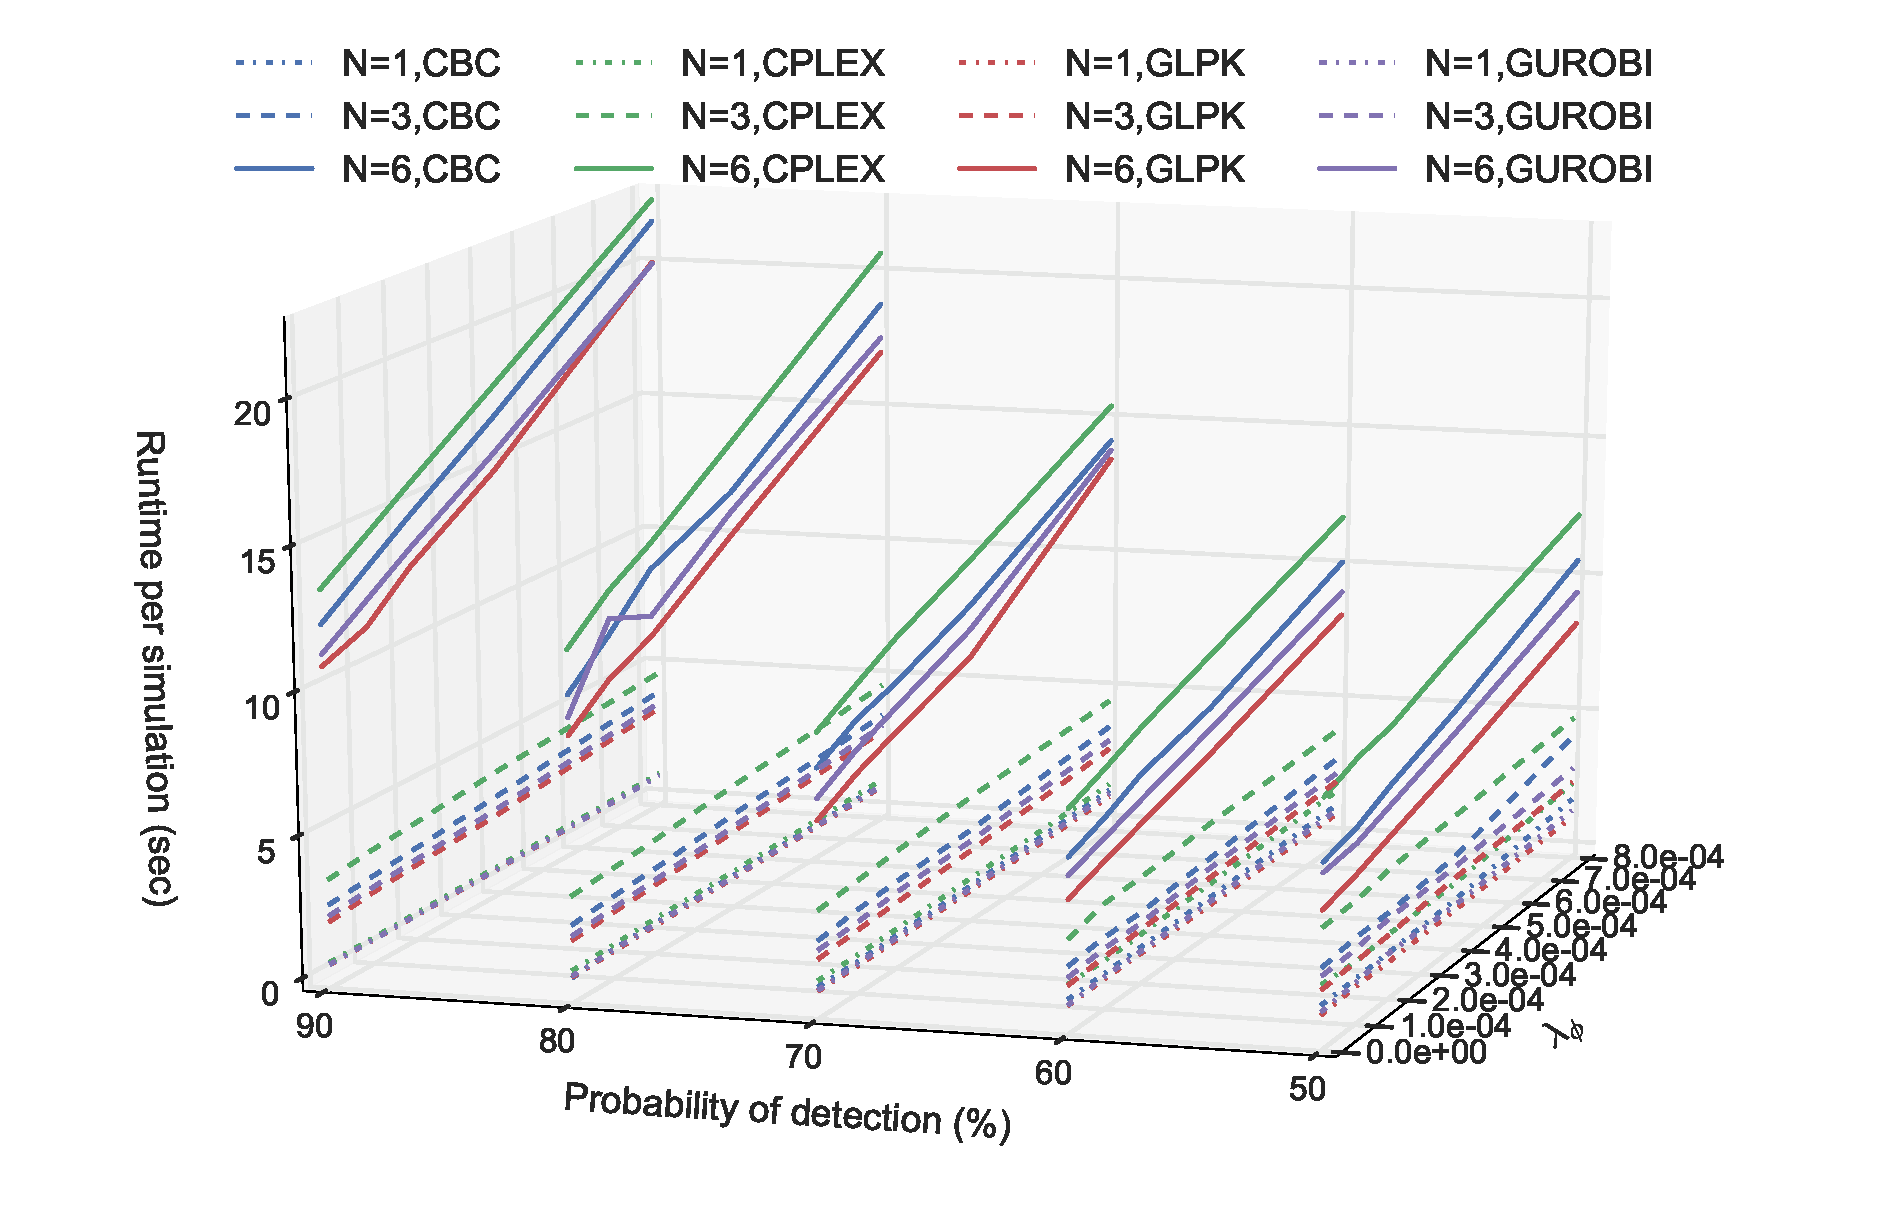
\includegraphics[clip, trim=0cm 1.5cm 0cm 0cm, width=\textwidth]{dynamic_agents_full_cooperation_cropped_runtime}
\caption{Scenario 1}
\label{fig:runtime_scenario_1}
\end{figure}
\begin{figure}[H]
\centering
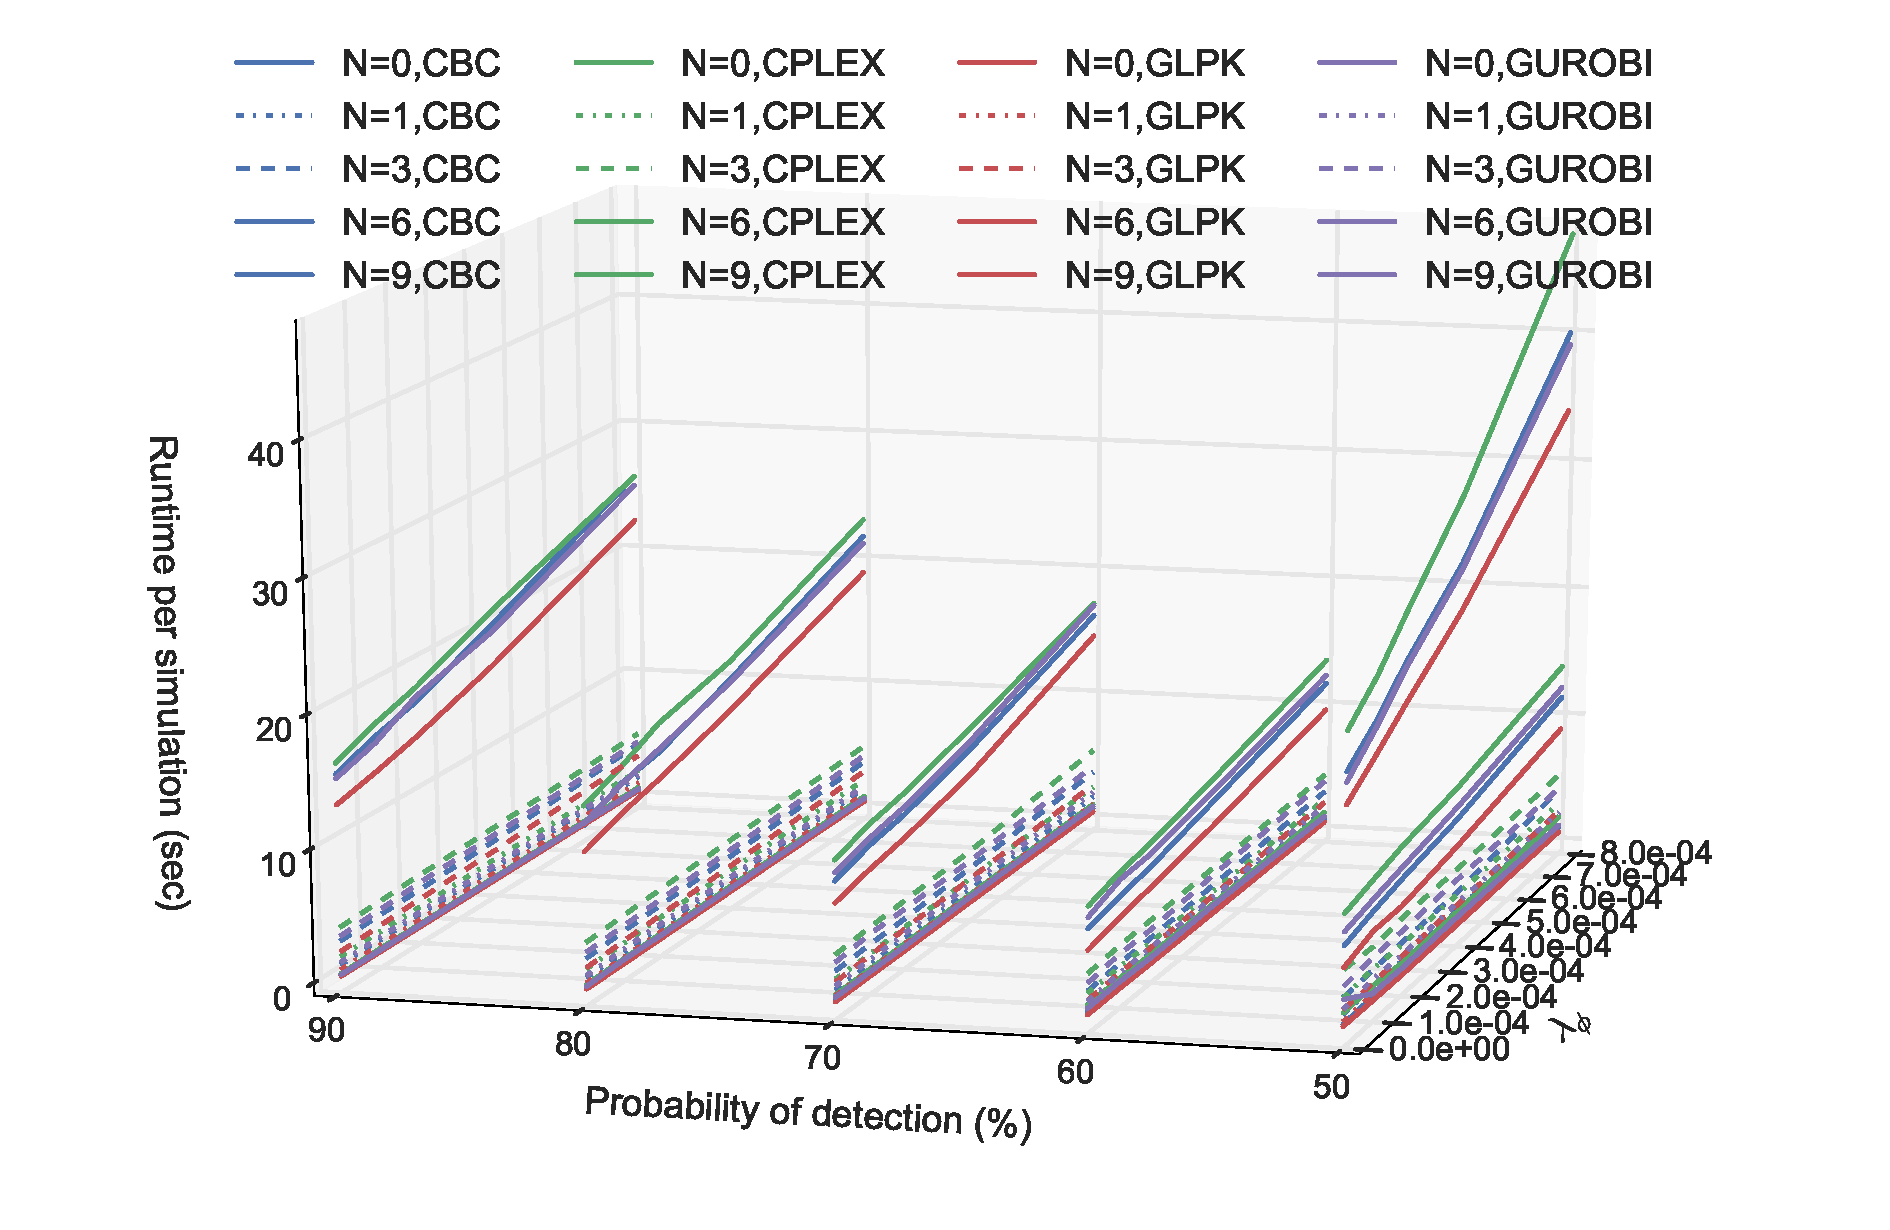
\includegraphics[clip, trim=0cm 1.5cm 0cm 0cm,width=\textwidth]{dynamic_agents_partial_cooporation_cropped_runtime}
\caption{Scenario 2}
\label{fig:runtime_scenario_2}
\end{figure}
\begin{figure}[H]
\centering
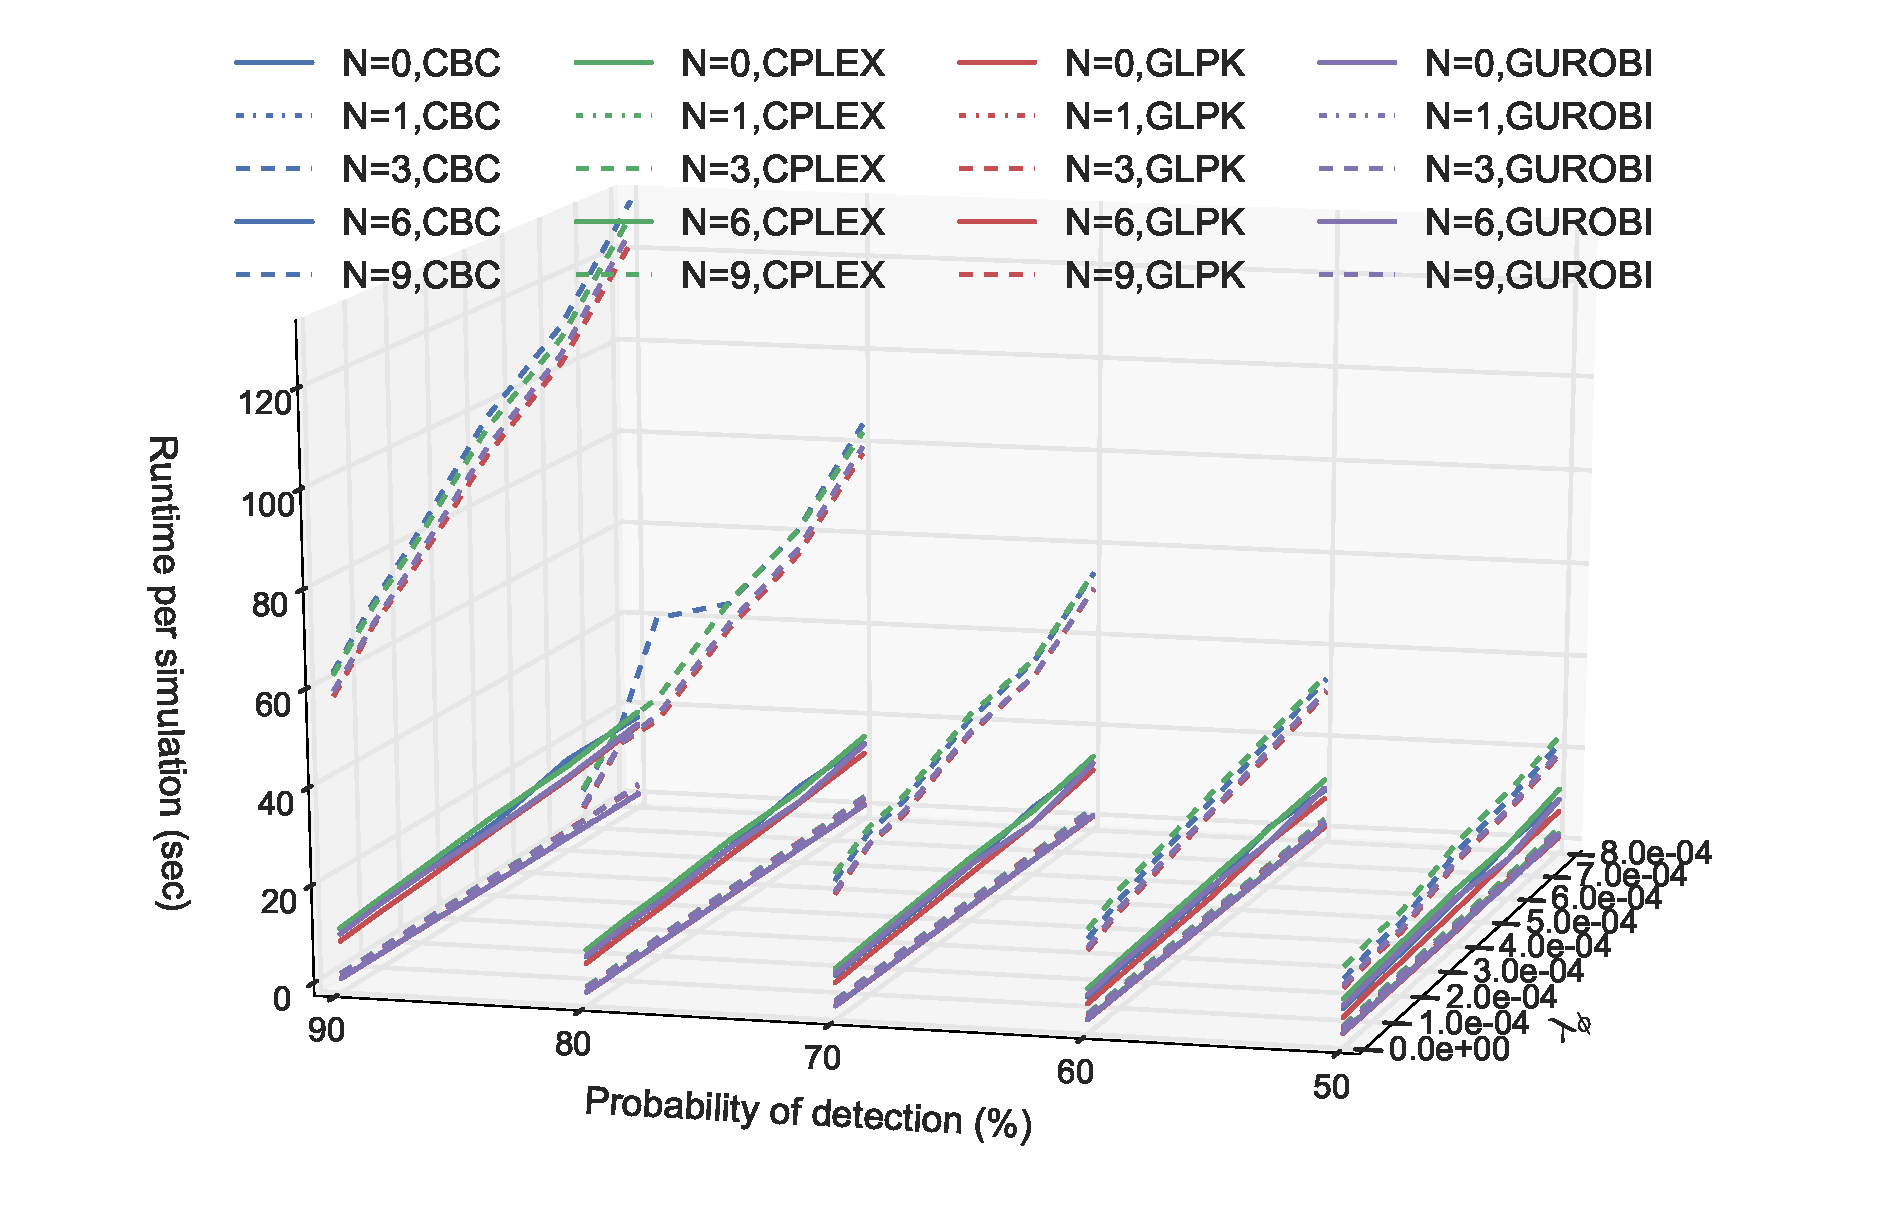
\includegraphics[clip, trim=0cm 1.5cm 0cm 0cm,width=\textwidth]{dynamic_and_static_agents_large_space_cropped_runtime}
\caption{Scenario 3}
\label{fig:runtime_scenario_3}
\end{figure}
\begin{figure}[H]
\centering
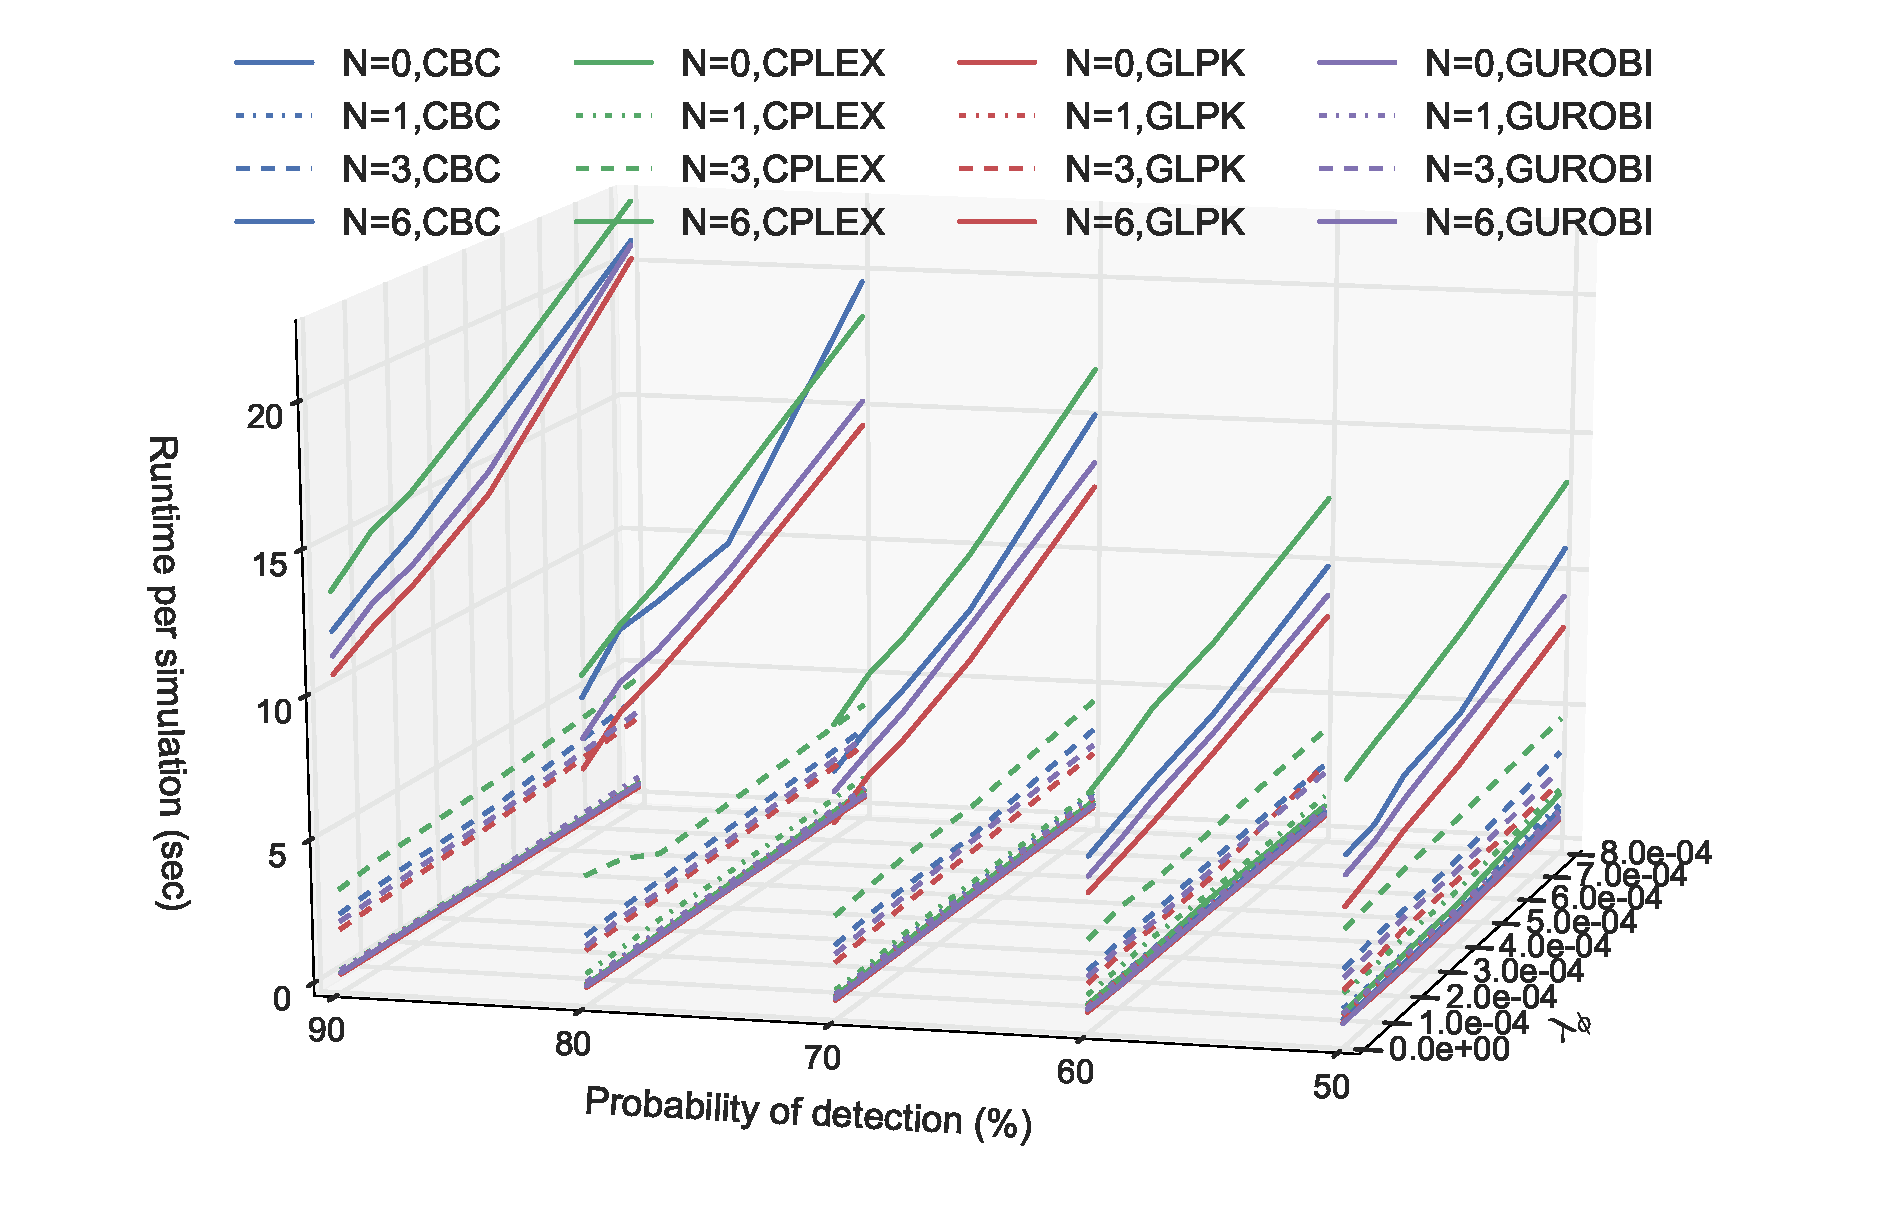
\includegraphics[clip, trim=0cm 1.5cm 0cm 0cm,width=\textwidth]{dynamic_and_static_agents_narrow_space_cropped_runtime}
\caption{Scenario 4}
\label{fig:runtime_scenario_4}
\end{figure}
\begin{figure}[H]
\centering
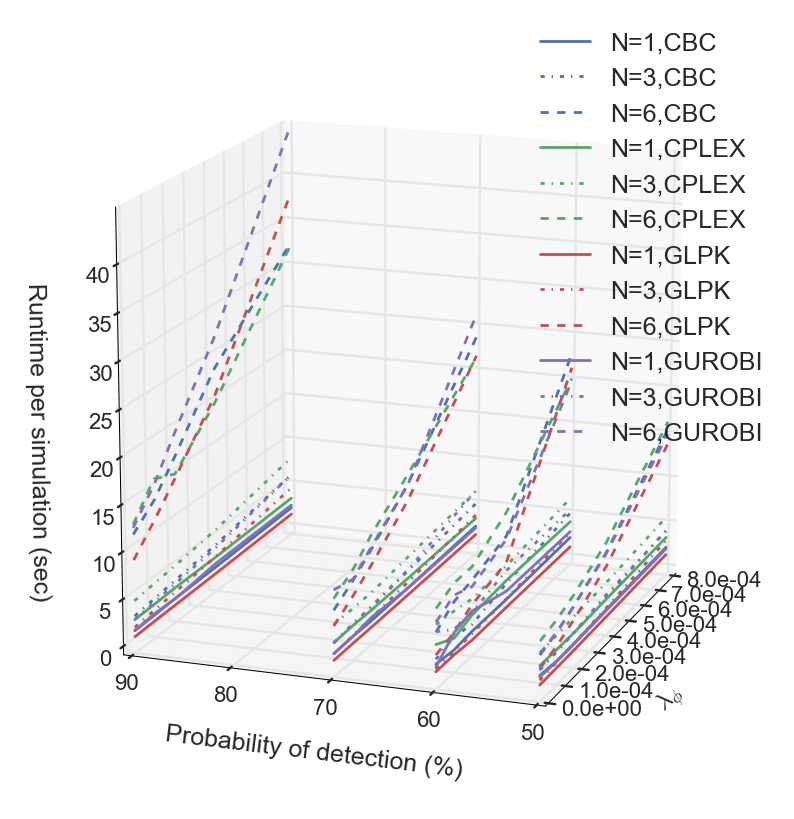
\includegraphics[clip, trim=0cm 1.5cm 0cm 0cm,width=\textwidth]{parallel_targets_cropped_runtime}
\caption{Runtime for scenario 5}
\label{fig:runtime_scenario_5}
\end{figure}